
\section{Konzept der statistischen Erwartung}

Das \textsl{Signifikanzniveau} $\alpha$ und die dazu komplementäre Wahrscheinlichkeit,
das \textsl{Vertrauensniveau} $1 - \alpha$ spielen eine zentrale Rolle bei der Bewertung
von Messergebnissen. Als wir in Kapitel~\ref{KonzepteinverseProbleme} die Konzepte der statistischen Auswertung
behandelt hatten,
haben wir diese beiden Begriffe gemeinsam mit dem des \textsl{Vertrauensintervalls} bzw.\
\textsl{Credible Interval} eingeführt, mit dem gemeinsamen Oberbegriff \textsl{Überdeckungsintervall}.
Es ist das Intervall, in dem mit einer Wahrscheinlichkeit von $P(X_1) = 1 - \alpha$ die
beobachteten Werte $X_{1,j}$ zur Größe $X_1$ liegen, das also die \glqq meisten\grqq
~Beobachtungen abdeckt.

Die Idee hinter dem Begriff des \textsl{Vertrauensintervalls} oder des \textsl{Credible Interval}s
ist, dass beim Bestimmen einer physikalischen Größe $X$ eine Vorstellung (eine Erwartung) darüber
existiert, wie die gemessenen oder beobachteten Werte verteilt sind. Das schließt die
Erwartung von Position und Breite des Bereichs, in dem die Werte liegen sollten, ein.
Diese Erwartung wird quantifiziert mit einer Angabe über die Wahrscheinlichkeit, dass die
zu messende Größe diesen oder jenen Wert annimmt, eher noch in welchem Bereich (Intervall) der
Wert zu erwarten ist. Wir \textsl{vertrauen} also darauf, dass wir einen Wert messen, der innerhalb eines
gewissen Intervalls liegen müsste, oder sagen, dass es plausibel oder \textsl{glaubwürdig}
(engl.\ \textsl{credible}) ist, dass die Beobachtungen in dem Intervall liegen.
Statt zu sagen, dass wir \textsl{eine Vorstellung haben}, können wir auch sagen,
dass wir \textsl{eine Hypothese aufstellen}. 


Code-Beispiel in Python (\href{https://mybinder.org/v2/gh/dhueser/MDA-Vorlesung-iprom-tu-bs/master?urlpath=/lab/tree/vorlesung/05_vorlesung/code/example_tTest.ipynb}{Klicke hier für interaktive Session}): 
\lstinputlisting[style=Python]{05_vorlesung/code/example_tTest.py}


Die Normalverteilung (Gaußverteilung) ist die grundlegende Verteilungsdichtefunktion
zur Beschreibung zufälliger Prozesse, beispielsweise Zerfallsprozesse und Diffusionsprozesse.
Bei rein stochastischen Prozessen wird von Zufallsgrößen ausgegangen, deren
Wahrscheinlichkeitsdichteverteilung eine Normalverteilung ist
\begin{equation}
p(X) \; = \; \frac{1}{\sqrt{2 \pi} \, \sigma} \, e^{-\frac{1}{2}\left(\frac{X - \mu}{\sigma}\right)^2}.
\end{equation}
Verteilungen wie die Poisson-Verteilung und die Binominal-Verteilung gehen für
unendlich viele Beobachtungen oder Stichprobenentnahmen in die Gaußverteilung über.

In der Wahrscheinlichkeitstheorie wird diese Tatsache exakt formuliert und ist der
\textsl{zentrale Grenzwertsatz} (engl.\ \textsl{central limit theorem}) CLT.
In einfacheren Worten können wir sagen:
\begin{quote}
Die Summe einer großen Anzahl von unabhängigen Zufallsgrößen folgt
asymptotisch einer stabilen Verteilung.
\end{quote}
Bei endlicher und positiver Varianz der Zufallsgrößen ist ihre Summe annähernd
normalverteilt, was die Sonderstellung der Normalverteilung erklärt.

Hierzu wird das Ziehen eines Wertes (das Machen einer Beobachtung) als Zufallsgröße
interpretiert.
Damit betrachten wir eine Stichprobe als Folge von Zufallsgrößen. Sind die Elemente
einer Stichprobe Zufallsgrößen, die
\textsl{unabhängig und identisch verteilt}, kurz u.i.v., sind, so ist auch ihre Summe
eine Zufallsgröße, die normalverteilt ist, wenn der Stichprobenumfang beliebig groß ist,
also gegen Unendlich konvergiert. In der englischsprachigen Literatur ist 
\textsl{unabhängig und identisch verteilt} unter dem Begriff
\textsl{independent and identically distributed}, kurz i.i.d., zu finden.

Liegt nun eine Einzelbeobachtung innerhalb der flachen
Ausläufer (\textsl{tails}) der Wahrscheinlichkeitsdichteverteilung,
also außerhalb des Vertrauensintervalls, so 
spricht man dann davon, dass der Wert (die Einzelbeobachtung)
signifikant von dem, was zu erwarten ist, abweicht. Das heißt, dass ein Ereignis eintritt,
das \textsl{nicht der Erwartung entspricht}. Somit \textsl{vermuten wir ein Problem}. Das Aufspüren
des Problems erfolgt durch \textsl{Hypothesentests}. Da die Normalverteilung
lange Ausläufer hat, gibt es eine kleine Wahrscheinlichkeit $\alpha$ dafür, dass es
weiter abseits liegende Werte gibt. Deshalb gilt es zu untersuchen,
ob solch ein Wert in der Tat im Rahmen der Normalverteilung weiter weg liegt
oder aber ob er auf Basis eines anderen Effektes gewonnen
wurde, ob er - statistisch formuliert - zu einer anderen Grundgesamtheit gehören könnte.

Der \textsl{Kolmogorow-Smirnow-Test} ist ein möglicher Test zum Prüfen, ob eine aus Beobachtungen
empirisch ermittelte Verteilung zu einer für die statistische Analyse der Beobachtungen
zugrundegelegten (erwarteten) Wahrscheinlichkeitsdichtefunktion passt.

% 30. Okt 2017

\section{Kolmogorow-Smirnow-Test}

\begin{figure}
\begin{center}
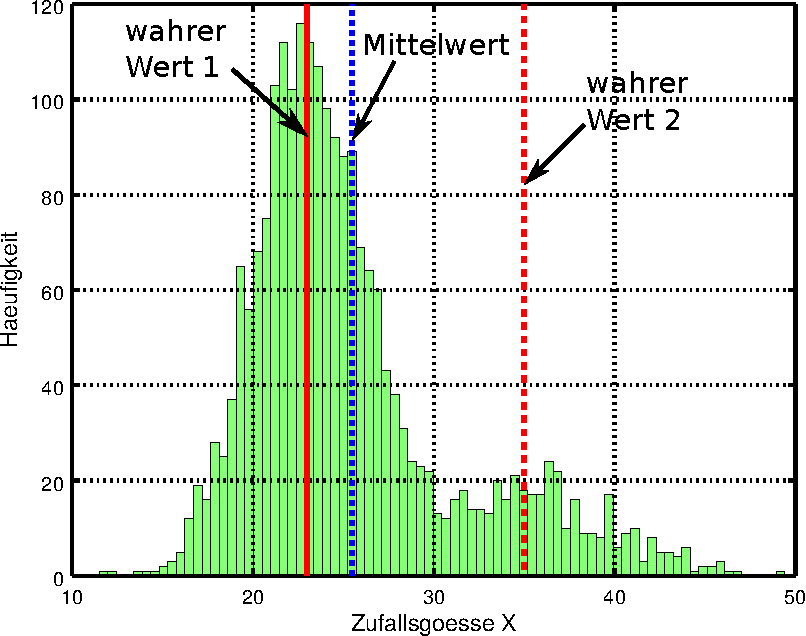
\includegraphics[width=80mm]{05_vorlesung/media/learn_robust.pdf}
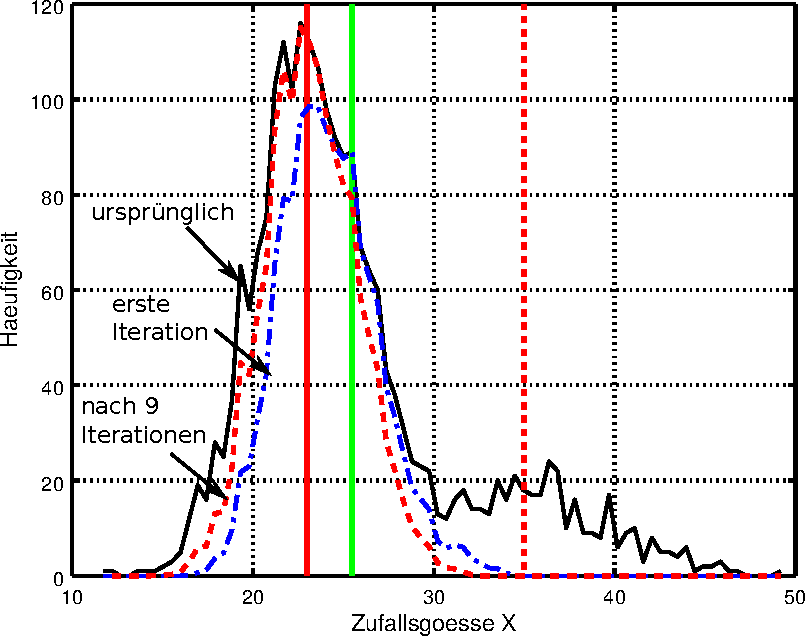
\includegraphics[width=80mm]{05_vorlesung/media/learn_robust_2.pdf}
\caption{Beispiel für nicht erwartungsgemäße Beobachtungen (\textsl{rechts}) und
Umgewichten um die Verteilungform der Normalverteilung anzupassen \textsl{links}}
\label{biasExample}
\end{center}
\end{figure}
Das in Abb.~\ref{biasExample} dargestellte Beispiel zeigt dieselben Diagramme und
Daten, die wir in Abschnitt~\ref{robustEstimation} bereits zur Veranschaulichung
robuster Schätzverfahren behandelt hatten. Den robusten Schätzverfahren liegt die
im folgenden erläuterte statistische Betrachtung zugrunde: Es liegt eine Annahme
(Hypothese) darüber vor, welcher Gestalt die Wahrscheinlichkeitsverteilung der
Beobachtungen ist und ob ein Reihe von Beobachtung zu einer gemeinsamen Verteilung
gehören oder zu unterschiedlichen Verteilungen. Technisch gesehen stellen sich die
Fragen, die statistisch formuliert lauten \glqq gehören Beobachtungen zu einer 
Verteilung\grqq ~oder \glqq gehören Beobachtungen zu mehreren verschiedenen Verteilungen\grqq,
als 
\begin{itemize}
\item \glqq stammen die Messwerte aus einem Prozess\grqq ~oder \glqq aus unterschiedlichen
Prozessen\grqq, 
\item \glqq werden alle Messwerte von demselben Effekt beeinflusst \grqq ~oder \glqq gibt es
für verschiedene Gruppen aus der Messreihe unterschiedliche beeinflussende Effekte\grqq.
\end{itemize}
Die Annahmen bzw.\ Hypothesen bezüglich der Verteilungen zur Wahrscheinlichkeit
von Beobachtungswerten werden geprüft. Diese Art der Prüfung wird \textsl{Hypothesentest}
genannt. Es gibt unterschiedliche Typen von Hypothesentests, einer davon ist 
der \textsl{Kolmogorow-Smirnow-Test}.
Er ist ein statistischer Test auf Übereinstimmung zweier Wahrscheinlichkeitsverteilungen.

Der Test verwendet die kumulierten Wahrscheinlichkeitsfunktionen
\begin{equation}
P(X) \; = \; \int\limits_{-\infty}^X \, p(X^\prime) \, \mathrm{d} X^\prime .
\end{equation}
Das hat den Vorteil, dass
die Verteilung der empirischen Häufigkeiten ohne Histogrammierung, d.h.\ ohne Einteilung in Klassen,
erfolgen kann.

Wir wollen damit prüfen, ob die Beobachtungen des in Abschnitt~\ref{robustEstimation} zur robusten
Schätzung betrachteten Beispiels der Annahme folgt, zu der Grundgesamtheit \textsl{genau einer}
Zufallsgröße $X_1$ zu gehören. Ferner nehmen wir an, dass ihre Ausprägungen (Beobachtungswerte)
unabhängig und identisch der Normalverteilung folgen.
\begin{quote}
Die Nullhypothese lautet:\\
Die Beobachtungen zu $X_1$ gehören zu einer
normalverteilten Grundgesamtheit.
\end{quote}
Wir prüfen, ob die Stichprobe $(X_{1,1}, X_{1,2}, \dots, X_{1,J})$ bezüglich
des Mittelwertes $y \, = \, \frac{1}{J} \sum_{j=1}^J X_{1,j}$ und der
empirischen Varianz $s^2 \, = \, \frac{1}{J-1} \sum_{j=1}^J (X_{1,j} \, - \, y)^2$ normalverteilt
ist. Die kumulierte Normalverteilung, mit der wir die kumulierte Verteilung der relativen Häufigkeiten
vergleichen, ist
\begin{equation}
P(X) \; = \;  \frac{1}{\sqrt{2\pi} s} 
\int\limits_{-\infty}^X \, e^{-\frac{1}{2}\left(\frac{X^\prime \, - \, y}{s}\right)^2} \, \mathrm{d} X^\prime .
\label{cdfKS}
\end{equation}
Die kumulierte Verteilung der relativen Häufigkeiten gewinnen wir darüber, dass wir die Werte der
Stichprobe in aufsteigender Reihenfolge sortieren
\begin{equation}
X_{1,k_1} \, \leq \, X_{1,k_2} \, \leq \,  \dots \, \leq \,  X_{1,k_J}
\end{equation}
Die Teilstichprobe mit der Beobachtung mit dem kleinsten Wert $(X_{1,k_1})$ hat die
relative kumulierte Häufigkeit $\frac{1}{J}$, die Teilstichprobe mit den zwei
kleinsten Beobachtungen $(X_{1,k_1}, X_{1,k_2})$ hat die relative kumulierte Häufigkeit $\frac{2}{J}$.
Die Teilstichprobe
\begin{equation}
(X_{1,k_1}, X_{1,k_2}, \dots, X_{1,k_j})
\qquad \mathrm{die~rel.~kum.~Haeufigk.} 
\qquad H(X_{1,k_j}) \; = \; \frac{j}{J}
\label{cdfH}
\end{equation}
\begin{figure}
\begin{center}
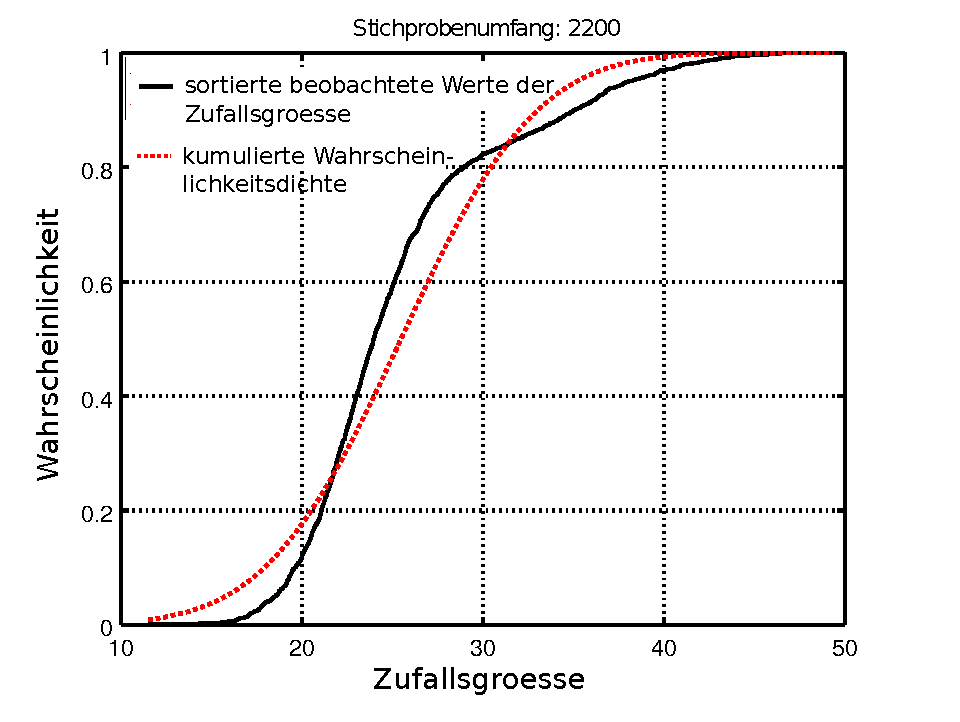
\includegraphics[width=100mm]{05_vorlesung/media/KS_pdf_iteration0.pdf}
\caption{\label{cdf4KStest} Vergleich der Wahrscheinlichkeiten (kumulierte Verteilungsdichten) aus der
empirische gewonnenen Häufigkeit der beobachteten Werte der Zufallsgröße
(schwarze, durchgezogene Kurve) mit der kumulierten Normalverteilung, die sich auf
die empirischen Erwartungswerte, den Mittelwert und die empirische Varianz, bezieht (rote,
gestrichelte Kurve).}
\end{center}
\end{figure}

Abb.~\ref{cdf4KStest} stellt zum Vergleich die Wahrscheinlichkeitsfunktion
(kumulierte Verteilungsdichte) $P(X)$ gemäß Gl.~(\ref{cdfKS})
als rote, gestrichelte Kurve und die kumulierte, relative Häufigkeit
$H(X_{1,k_j}) \; = \; \frac{j}{J}$
als schwarze, durchgezogen gezeichnete Kurve in einem Diagramm dar.


Die Prüfgröße des \textsl{Kolmogorow-Smirnow}-Tests ist
\begin{equation}
\arraycolsep=2.4pt\def\arraystretch{2}
\begin{array}{l}
\sup\limits_{X} \mid H(X_{1,k_j}) \, - \, P(X) \mid \; = \;\\
\max\limits_{k_j} \left\{ \max \left\{ \mid H(X_{1,k_j}) \, - \, P(X_{1,k_j}) \mid, \;
\lim\limits_{X \rightarrow X_{1,k_j}} \mid H(X) \, - \, P(X_{1,k_j} - 1) \mid \right\} \; \right\} .
\end{array}
\end{equation}
Dabei steht sup für Supremum, was \textsl{kleinste, obere Schranke} heißt.
Zu jeder Ausprägung der Stichprobe wird der Betrag der beiden Wahrscheinlichkeitsverteilungen
gebildet. Die Berechnung des Grenzwertes
$\lim\limits_{X \rightarrow X_{1,k_j}} \mid H(X) \, - \, P(X_{1,k_j} - 1) \mid$
für das Supremum ist erforderlich, wenn die kumulierte relative Häufigkeit
(Summenhäufigkeit) durch Kumulieren eines Histogramms, also einer in Klassen
quantisierten Stichprobe, berechnet wurde. Dabei soll die Schreibweise mit
dem Grenzwert $\lim\limits_{X \rightarrow X_{1,k_j}} \mid H(X) \, - \, P(X_{1,k_j} - 1) \mid$
zum Ausdruck bringen, dass man infinitesimal dicht aber doch prinzipiell rechts 
von $X_{1,k_j}$ an der Stufe ist, praktisch wird aber direkt
$\mid H(X_{1,k_j}) \, - \, P(X_{1,k_j} - 1) \mid$
berechnet. Für die nichtklassierte, sortierte Stichprobe berechnen wir einfach nur
\begin{equation}
\max\limits_{k_j} \left\{ \mid H(X_{1,k_j}) \, - \, P(X_{1,k_j}) \mid \right\} .
\end{equation}

Die Wahrscheinlichkeit, dass die Beobachtungen nicht zur in der Hypothese angenommenen
Verteilung passt, ist die Wahrscheinlichkeit, dass die Beobachtung
in den Ausläufern (\textsl{Tails}) der Dichteverteilung liegt, weshalb wir
die durch die Fläche in den Tails repräsentierte Wahrscheinlichkeit mit
\textsl{Signifikanzniveau} $\alpha$ bezeichnen.

Beim Kolmogorow-Smirnow-Test wird die Nullhypothese verworfen, wenn
die empirische relative Häufigkeit einen Grenzwert überschreitet,
der vom Signifikanzniveau $\alpha$ und dem Stichprobenumfang $J$ abhängt
\begin{equation}
\sup\limits_{X} \mid H(X_{1,k_j}) \, - \, P(X) \mid \; > \; K_{\alpha, J}
\end{equation}
wobei es zu Schwellwerten $K_{\alpha, J}$ für $J < 35$ Tabellen in den gängigen
Formelsammlungen gibt und
für $J \geq 35$ folgende Näherung verwendet wird:
\begin{equation}
K_{\alpha, J} \; = \; \sqrt{-\frac{1}{2 \, J} \, \ln(\frac{\alpha}{2})}
\label{KSpruefgroesse}
\end{equation}


\section{Wahrscheinlichkeitsdichtefunktionen und ihre Parameter}

Bei vielen beobachteten Stichproben, die signifikant von dem Modell, das besagt, dass sie zu genau einer
normalverteilten Grundgesamtheit gehören, abweichen, handelt
es sich um Beobachtungen aus Prozessen, denen mehrere überlagerte stochastische Anteile
zugrunde liegen. Bei dem in Abb.~\ref{biasExample} illustrierten Beispiel waren dies
zwei normalverteilte Grundgesamtheiten mit verschiedenen Erwartungswerten $\mu_1$ und
$\mu_2$ und mit unterschiedlichen Varianzen $\sigma^2_1$ und $\sigma^2_2$.

Für eine Bewertung von gemessenen Werten einer Größe, d.h.\ von Beobachtungen, werden statistische
Modelle zugrunde gelegt. Ein statistisches Modell zu beobachtbaren Größen umfasst die 
Vorstellung von Zufallsgrößen und der Verteilung ihrer Beobachtungswerte.
Wahrscheinlichkeitsdichtefunktionen werden parametrisiert über ihre statistischen Momente.
Diese charakterisieren den Kurvenverlauf der Funktion hinsichtlich ihrer Lage, Breite,
Symmetrie und so weiter.

Der \textsl{Erwartungswert einer Zufallsgröße} $X$ ist das erste statistische Moment
der Verteilungsdichte $p$ ihrer Grundgesamtheit
\begin{equation}
\mathrm{E}(X) \; = \; \int\limits_{-\infty}^{\infty} \, X \, p(X) \, \mathrm{d} X \; =: \; \mu^{(1)}(X)
\end{equation}
das ihren Schwerpunkt angibt.
Der Erwartungswert der \textsl{Varianz}
einer Zufallsgröße $X$ entspricht dem zweiten statistischen Moment
der Verteilungsdichte $p$.
Das zweite statistische Moment ist definiert durch
\begin{equation}
\int\limits_{-\infty}^{\infty} \, X^2 \, p(X) \, \operatorname{d} X \; =: \; \mu^{(2)}(X)
\end{equation}
und die Varianz ist das zweite Moment der um den Erwartungswert verschobenen Zufallsgröße
\begin{equation}
\operatorname{Var}(X) \; = \; \int\limits_{-\infty}^{\infty} \, (X - \operatorname{E}(X))^2 \,
 p(X) \, \mathrm{d} X
\end{equation}
deren Wurzel
\begin{equation}
\sigma \; = \; \sqrt{\operatorname{Var}(X)}
\end{equation}
ein Maß für die Breite von $p$ darstellt.
Die Schiefe einer Verteilungsdichte wird durch das dritte statistische Moment
\begin{equation}
\int\limits_{-\infty}^{\infty} \, X^3 \, p(X) \, \mathrm{d} X \; =: \; \mu^{(3)}(X)
\end{equation}
gewonnen, bei dem die Zufallsgröße um ihren Erwartungswert verschoben und auf die Wurzel ihrer
Varianz normiert
\begin{equation}
\operatorname{Skew}(X) \; = \; \int\limits_{-\infty}^{\infty} \, \left(\frac{X - \mathrm{E}(X)}{\sigma}
\right)^3 \, p(X) \, \operatorname{d} X
\end{equation}
wird. Das dritte statistische Moment der normierten Zufallsgröße heißt
\textsl{Skewness}.

Ein Maß für die Überhöhung oder Abflachung relativ zur Normalverteilung wird durch
das vierte statistische Moment
\begin{equation}
\int\limits_{-\infty}^{\infty} \, X^4 \, p(X) \, \mathrm{d} X \; =: \; \mu^{(4)}(X)
\end{equation}
gewonnen wird, bei dem die Zufallsgröße um ihren Erwartungswert verschoben und auf die Wurzel ihrer
Varianz normiert
\begin{equation}
\operatorname{Kurt}(X) \; = \;  \int\limits_{-\infty}^{\infty} \, \left(\frac{X - \operatorname{E}(X)}{\sigma}
\right)^4 \, p(X) \, \operatorname{d} X
\end{equation}
wird. Das vierte statistische Moment der normierten Zufallsgröße heißt
\textsl{Kurtosis}.

% ======

%Die Kombination der Wahrscheinlichkeitsverteilungen von mehreren unabhängigen kontinuierlichen
%Zufallsgrößen $X_1, \dots, X_N$ haben wir in den vergangenen Vorlesungen bereits kennengelernt,
%als wir die Berechnung der Likelihood und der Posterior besprochen haben.
%Bei der Likelihood wurde jede Beobachtung als von jeder anderen Beobachtung unabhängige
%Zufallszahl mit gleichen Varianzen (identische Verteilungen) behandelt.
%Beim Posterior wurden die Größen, zu
%denen als {`a} priori Informationen ein Erwartungswert und eine Varianz gegeben sind,
%als jeweilige Zufallsgrößen behandelt. Mit Zufallsgrößen $X_1, \dots, X_N$ können
%auch verschiedene Messgrößen sein, wie beispielsweise Strom und Widerstand (hier $N=2$),
%oder drei Koordingaten im Raum ($N=3$), oder zwei Positionskoordinaten auf einem CCD-Chip
%gemeinsam mit dem jeweiligen Intensitätswert ($N=3$).

%Gegeben seien $N$ Zufallsgrößen $X_1, \dots, X_N$ und zu jeder Zufallsgröße
%sei eine Wahrscheinlichkeitsdichteverteilung $p(X_i)$ mit $i=1,\dots,N$ gegeben.
%Dabei sei $p$ eine beliebige Verteilung. Sie muss keine Normalverteilung sein.
%Die Zufallsgrößen seinen kontinuierlich, es gelte $X_i \in I \!\! R$ und für den Zufallsvektor
%$\mathrm{X} = (X_1, \dots, X_N) \in I \!\! R^n$.
%Dann gilt unter der Voraussetzung, dass sie unabhängig voneinander sind, für die gemeinsame Wahrscheinlichkeitsdichteverteilung $p(X_1, \dots, X_N)^\mathsf{T} = p(\mathbf{X})$:
%\begin{equation}
%p(\mathrm{X}) \; = \;
%\frac{1}{\int\limits_{-\infty}^{+\infty} \dots \int\limits_{-\infty}^{+\infty}
%\prod\limits_{i=1}^N p(X_i^\prime) \mathrm{d} X_1^\prime \dots \mathrm{d} X_N^\prime}
%\prod\limits_{i=1}^N p(X_i) .
%\end{equation}
%Wir wollen uns die Verteilung für zwei Zufallsgrößen, also $\mathbf{X}^\mathsf{T} = (X_1,X_2)$,
%für den Fall, dass beide Zufallgrößen normalverteilt seien genauer anschauen
%\begin{equation}
%p(\mathbf{X}) = \frac{1}{2 \pi \sigma_1 \sigma_2} \,
%e^{-\frac{1}{2} \, 
%  \left(\frac{X_1-\mu_1}{\sigma_1}\right)^2
%  \, - \, \frac{1}{2} \,  \left(\frac{X_2-\mu_2}{\sigma_2}\right)^2}
%\end{equation}

% 6. Nov. 2017

\section{Vertrauensintervall und t-Verteilung}

Wir hatten bereits in Kapitel \ref{KonzepteinverseProbleme} angesprochen, wie
\textsl{Vertrauensintervall} $[x_1, x_2]$, Wahrscheinlichkeistdichtefunktion $p$,
\textsl{Signifikanzniveau} $\alpha$ und \textsl{Vertrauensniveau} $1-\alpha$ zusammen hängen.
Das Vertrauensintervall gibt den Bereich an, in dem ein Ereignis mit 
Wahrscheinlichkeit $1-\alpha$ beobachtet wird bzw.\ die Messgröße einen Wert in diesem Bereich
annimmt, also
\begin{equation}
\int\limits_{x_1}^{x_2} p(X) \, \operatorname{d} X \; = \; 1 - \alpha .
\end{equation}
Eine Wahrscheinlichkeitsdichteverteilung $p(X)$
wird immer so normiert, dass ihre Fläche $1$ ist:
\begin{equation}
\int\limits_{-\infty}^\infty p(X) \, \operatorname{d} X \; = \; 1
\end{equation}
Das heißt mit anderen Worten:
Unsere Größe nimmt mit Wahrscheinlichkeit $1$ irgend einen beliebigen
Wert zwischen minus und plus Unendlich an.

Auch hatten wir in Kapitel \ref{KonzepteinverseProbleme} durchgenommen, wie man aus unterschiedlichen vorliegenden
Informationen eine Wahrscheinlichkeitsdichteverteilung berechnet, um den
Erwartungswert
\begin{equation}
E(X) \; = \; \int\limits_{-\infty}^\infty \, X  p(X) \, \operatorname{d} X
\end{equation}
zu bestimmen und um aus der Umkehrfunktion $P^{-1}$ der kumulativen Verteilung
das Über\-deck\-ungs\-intervall 
\begin{equation}
[P^{-1}(\frac{\alpha}{2}), P^{-1}(1-\frac{\alpha}{2})]
\end{equation}
zu ermitteln.

Man kann zur Berechnung eines Überdeckungsintervalls
rechenzeiteffizient auf vorhandene tabellierte Werte für
die Umkehrfunktion der Normalverteilung zurück greifen, wenn
folgendes der Fall ist:
\begin{itemize}
\item Über die reinen Beobachtungen $X_{1,j}$ hinaus liegen keine
Informationen vor, also keine vorherigen Ergebnisse zu den zu
schätzenden Modellparameter (kein \textsl{Prior})
und keine weiteren beeinflussenden Verteilungen. 
\item Es kann davon ausgegangen werden, dass die Streuung der
einzelnen Beobachtungswerte um das Modell
normalverteilt sind.
\end{itemize}
Für kleine
Stichprobenumfänge wird eine der Normalverteilung ähnliche Verteilung
herangezogen, die je kleiner der Stichprobenumfang ist, um so stärker ausgeprägte
Ausläufer (\textsl{Tails}) hat, die $t$-Verteilung. Diese werden wir im Laufe
dieses Kapitels beleuchten.

Zunächst erörtern wir die Berechnung der Vertrauensintervalle auf Basis
tabellierter Werte von Integrationsgrenzen zu ausgesuchten Ver\-trauens\-niveaus
der Normalverteilung. Eine solche Integrationsgrenze wird \textsl{Quantil}
genannt. Die Tabellen beziehen sich auf normierte Zufallsgrößen.
Für die Gaußverteilung normieren wir die Zufallsgröße, so dass der
Erwartungswert $\mu = 0$ ist und die Varianz $\sigma^2 = 1$, d.h.
$Z$ ist \textsl{standardnormalverteilt}
\begin{equation}
Z \; \sim \; \mathcal{N}(0,1) .
\label{standardNormalverteilt}
\end{equation}
Die Wahrscheinlichkeitsdichtefunktion $p(Z)$ ist die \textsl{Standard}normalverteilung 
\begin{equation}
p(Z) \; = \; \frac{1}{\sqrt{2 \pi}} \, e^{-\frac{1}{2} Z^2}
\qquad \textrm{mit} \qquad Z \; = \; \frac{X - \mu}{\sigma} .
\end{equation}

Die in den Formelsammlungen und Tabellenwerken aufgelisteten Grenzen sind
als obere Integrationsgrenze definiert
\begin{equation}
\int\limits_{-\infty}^{z_\alpha} p(Z) \mathrm{d} Z \; = \; \alpha .
\label{WahrscheinlichkeitQuantil}
\end{equation}
In Abb.~\ref{normVertQuantil} wird dies anhand des Quantils $z_\alpha = 0.5244$ 
zu $\alpha = 0.7$ also $70 \%$ Wahrscheinlichkeit beispielhaft gezeigt.

\begin{figure}
\begin{center}
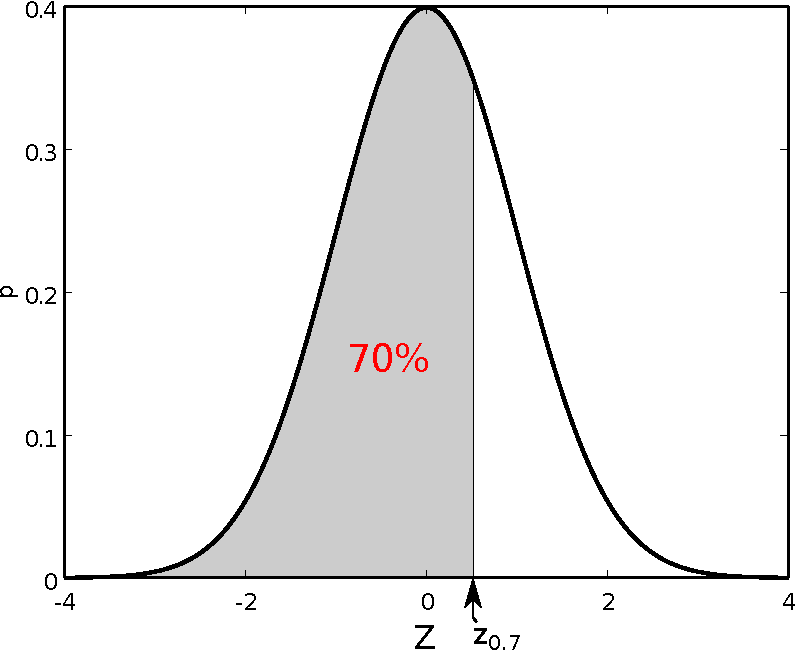
\includegraphics[width=79mm]{05_vorlesung/media/normpdfQuantil.pdf}
\hspace{5mm}
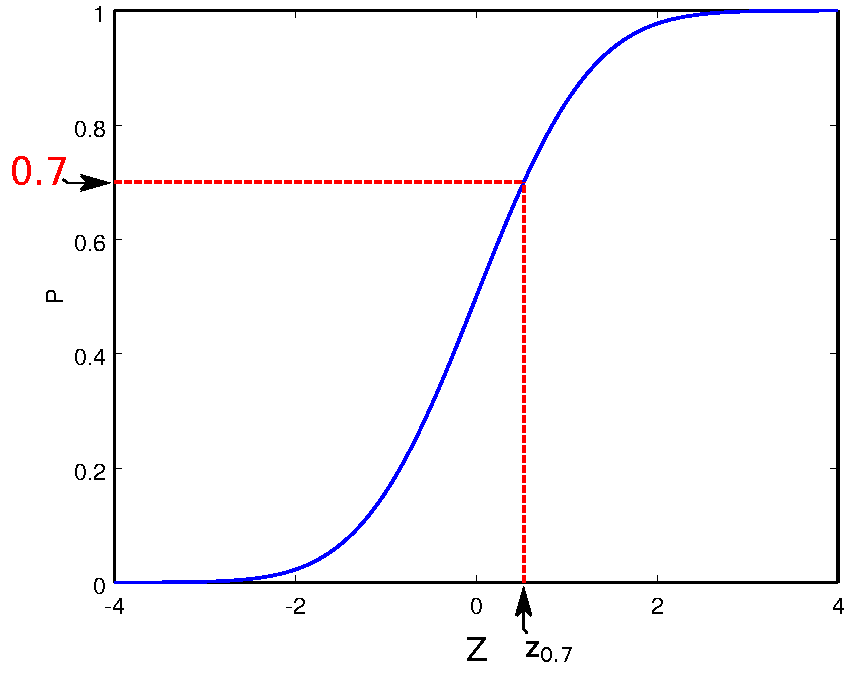
\includegraphics[width=81mm]{05_vorlesung/media/normcdfQuantil.pdf}
\caption{\label{normVertQuantil} Quantil $z_\alpha = 0.5244$ und Wahrscheinlichkeit 
$\alpha = 0.7$ der Standard\-normalverteilung.}
\end{center}
\end{figure}

Dies lesen wir so:
\begin{quote}
Die Ereignisse Werte zu $Z$ zu beobachten, die kleiner sind als $z_\alpha$, können
mit einer Wahrscheinlichkeit von $\alpha$ eintreten.
\end{quote}
Die in den Tabellenwerken gelisteten Wahrscheinlichkeiten $\alpha$ werden
aus der Integration der Wahrscheinlichkeitsdichte der normierten Zufallsgröße
von minus Unendlich bis zu einer endlichen oberen Integrationsgrenze $z_\alpha$
gewonnen.
Die zu einem Wert eines Quantils gehörende Wahrscheinlichkeit wird durch den tiefgestellten
Index bei $z_\alpha$ gekennzeichnet, in unserem Beispiel aus Abb.~\ref{normVertQuantil}
ist dies dann
$$
z_{0.7} \; = \; 0.5244
$$
Als weiteres Beispiel betrachten wir die Frage, wie hoch die Wahrscheinlichkeit ist,
Werte zu beobachten, die in den Ausläufern einer Verteilungsdichte liegen.
Die Ausläufer werden im Englischen
als \textsl{Tails} (Schwänze) bezeichnet. Dies sollen Beobachtungen zu der normierten
Zufallsgröße $Z$ mit Werten, die zum einen kleiner oder gleich $-1.960$ sind, sein
$$
z_{0.025} \; = \; -1.960
$$
und zum anderen, die Beobachtungen mit Werten größer oder gleich $1.960$, also die
in dem rechten Ausläufer (\textsl{Tail}) der Standardnormalverteilung liegen.
Die Wahrscheinlichkeit für Beobachtungen im linken \textsl{Tail} ist
\begin{equation*}
\int\limits_{-\infty}^{-1.960} p(Z) \mathrm{d} Z \; = \; 0.025 .
\end{equation*}

Aufgrund der Symmetrie der Standardnormalverteilung ist die Wahrscheinlichkeit für das Liegen von
Werten im rechten \textsl{Tail} ebenfalls $0.025$. Wir rechnen also zusammen, dass mit
einer Wahrscheinlichkeit von $0.05 = 0.025+0.025$ Werte in den beiden \textsl{Tails} außerhalb
des Intervalls $[-1.960, 1.960]$ liegen können. Somit ist die Wahrscheinlichkeit, dass sie
innerhalb des Intervalls liegen $1 - 0.05 = 0.95$
\begin{equation}
\int\limits_{-1.96}^{1.96} \, p(Z) \, \operatorname{d} Z \; = \; 0.95
\end{equation}
was uns zeigt, wie wir die Tabellen zu verwenden haben.
Wenn wir ein zweiseitiges Intervall betrachten wollen, wie hier zu einem Vertrauensniveau
von $95 \%$, so müssen wir im Tabellenwerk nach dem Quantil, das für $97.5 \%$ gelistet
ist, schauen
$$
z_{0.975} \; = \; 1.960
$$
weil
$$
0.95 \; = \; 
\underbrace{\int\limits_{-\infty}^{z_{0.975}} \, p(Z) \, \operatorname{d} Z}_{0.975} \; - \;
\underbrace{\int\limits_{-\infty}^{z_{0.025}} \, p(Z) \, \operatorname{d} Z}_{0.025}
$$
Aufgrund der Achssymmetrie der Normalverteilung gilt 
$$
z_{\frac{1}{2}\alpha} = -z_{1-\frac{1}{2}\alpha} .
$$
Da sich die Quantile zum jeweiligen Vertrauensniveau $1-\alpha$ auf die normierte Zufallsgröße
beziehen, muss für die Berechnung des Vertrauensintervall zurückgerechnet werden
\begin{equation}
Z \; = \; \frac{X - \mu}{\sigma} \qquad \Leftrightarrow \qquad X \; = \; \mu + Z \sigma
\end{equation}
also
\begin{equation}
[z_{\frac{1}{2}\alpha}, z_{1-\frac{1}{2}\alpha}] = 
[-z_{1-\frac{1}{2}\alpha}, z_{1-\frac{1}{2}\alpha}]
 \qquad \Leftrightarrow  \qquad
[\mu \, - \, z_{1-\frac{1}{2}\alpha} \, \sigma, \mu \, + \, z_{1-\frac{1}{2}\alpha} \, \sigma]
\end{equation}
Mit $\alpha$ sind die $5 \%$ und mit $1-\alpha$ die $95 \%$ Vertrauensniveau gemeint.

Die Likelihood wird maximal für
\begin{equation}
y \; = \; \frac{1}{J} \sum_{j=1}^J X_{1,j} ,
\end{equation}
wobei $y$ der Schätzwert für den Modellparameter $Y$ ist.
Der Schätzwert $s^2$ für die Varianz $\sigma^2$ wird berechnet mit
\begin{equation}
s^2 \; = \; \frac{1}{J-1} \sum_{j=1}^J (X_{1,j} - y)^2 .
\end{equation}

Nachdem wir gesehen haben, wie wir für eine normalverteilte Zufallsgröße
das Vertrauensintervall ermitteln können, wenden wir uns jetzt der Thematik zu,
wenn wir zu einer Zufallsgröße nur relativ wenige Beobachtungen haben.

%------------------- kleine Stichprobenumfaenge -> Motivation t-Verteilung
\begin{figure}
\begin{center}
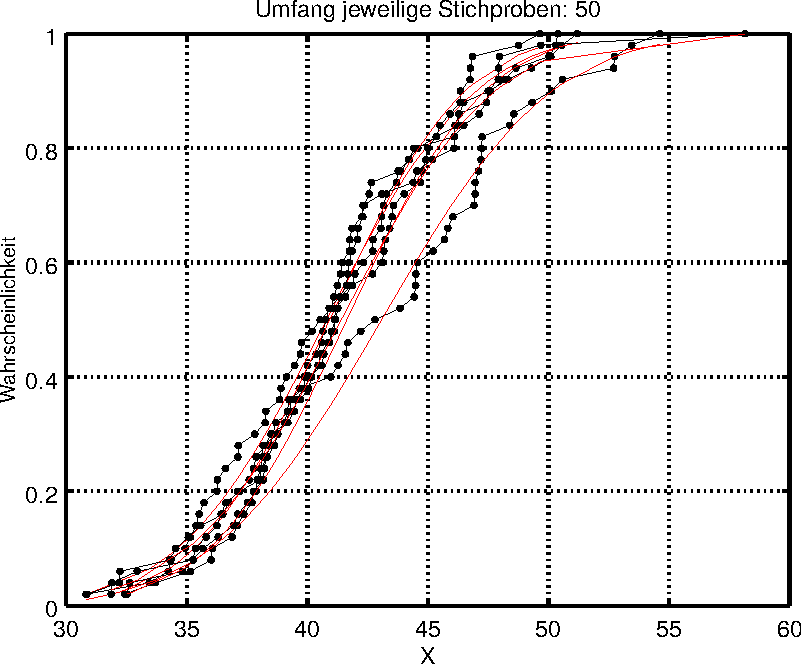
\includegraphics[width=100mm]{05_vorlesung/media/learn_Student_t1samples.pdf}
\caption{\label{kumulWahrsch} Kumulative relative Wahrscheinlichkeitsfunktionen und relative
Summenhäufigkeiten von verschiedenen Stichproben mit jeweils $J \, = \ 50$ Werten, entnommen aus einer
Grundgesamtheit mit $\mu \, = \, 42$ und $\sigma \, = \, 5$.}
\end{center}
\end{figure}
Wenn wir aus einer sehr großen Stichprobe, die einer Grundgesamtheit entnommen wurde,
disjunkte Teilstichproben von kleinerem Umfang ($J < 100$) in Grüppchen unterteilen, so können wir
beobachten, dass sowohl die Mittelwerte streuen als auch die Varianzen.
Diese Grüppchen oder Teilstichproben können wir als mehrere Stichproben aus einer normalverteilten
Grundgesamtheit ansehen. 
Abb.~\ref{kumulWahrsch} illustriert wie unterschiedlich die Verteilungsfunktionen von
Stichproben mit relativ kleinem Umfang ($J \, = \ 50$) aussehen können, obwohl sie zu derselben
Grundgesamtheit gehören. Dieses Beispiel wurde wie folgt mit Gnu-octave generiert:
\begin{verbatim}
function example_t()
  J1 = 50;
  mu1 = 42;
  sigma1 = 5;
  samples = [];
  for kappa = 1:5
    samples = [samples  (mu1 + sigma1*randn(J1,1))];
  end
  figure(3000); hold on;
  [J1, nS] = size(samples);
  for kappa = 1:5
    [P, H, xsort, xbar, s] = cumulatives(samples(:,kappa));
    plot( xsort, H, 'k.-');
    plot( xsort, P, 'r-');
  end
  xlabel('X', 'fontsize', 14);
  ylabel('Wahrscheinlichkeit', 'fontsize', 12);
  title(['Umfang jeweilige Stichproben: ' num2str(J1)], 'fontsize', 14);
  grid on;
  set(gca, 'fontsize', 14, 'linewidth', 2);
  hold off;
end
function [P, H, xsort, xbar, s] = cumulatives(x)
  xbar = mean(x);
  s = std(x);
  J1 = length(x);
  [xsort, isort] = sort(x, 'ascend');
  H = [1:J1]'/J1;
  P = normcdf( xsort, xbar, s);
end
\end{verbatim}
Zur Bewertung der Flachheit bzw.\ Ausgeprägtheit der Ausläufer einer Verteilung berechnen wir
ihre \textsl{Kurtosis}. Die \textsl{Kurtosis} der Normalverteilung hat den Wert $3$. 

Die empirischen Schätzer für den Erwartungswert, die Varianz, die Skewness und Kurtosis
berechnen wir aus einer Stichprobe mit Beobachtungswerten $X_{1,1}, \dots, X_{1,J}$
wie folgt:
\begin{itemize}
\item[] Der Mittelwert wird berechnet mit
\begin{equation}
y \; = \; \frac{1}{J}\sum_{j=1}^J \, X_{1,j} .
\end{equation}
\item[] Die empirische Standardabweichung wird berechnet mit
\begin{equation}
s \; = \; \sqrt{ \frac{1}{J-1}\sum_{j=1}^J \, (X_{1,j} - y)^2 }.
\label{empirischeStd}
\end{equation}
Zu bemerken ist, dass jetzt durch $J-1$ und nicht durch $J$ geteilt wird, weil
das $y$ aus den Werten der Stichprobe $X_{1,1}, \dots, X_{1,J}$ gewonnen wurde und somit
die Anzahl der Freiheitsgrade $\nu$ um Eins verringert wird, also $\nu = J-1$.
\item[] 
Die empirische Skewness wird berechnet mit
\begin{equation}
\textrm{skew} \; = \; \frac{1}{J} \sum_{j=1}^J \, \left( \frac{X_{1,j} - y}{s} \right)^3 .
\end{equation}
\item[] Die empirische Kurtosis wird berechnet mit
\begin{equation}
\textrm{kurt} \; = \; \frac{1}{J} \sum_{j=1}^J \, \left( \frac{X_{1,j} - y}{s} \right)^4 .
\end{equation}
\end{itemize}
Bei dem in Abb.~\ref{kumulWahrsch} gezeigten Beispiel mit mehreren Stichprobenentnahmen aus
einer Grundgesamtheit erhalten wir folgende aus den Momenten abgeleiteten empirischen 
Parameter der Verteilungen:
\begin{center}
Tabelle 1:

\begin{tabular}{c||c|c|c|c}
\hline
\multicolumn{5}{c}{Einzelstichproben, Umfang jeweils $J = 50$}\\
\hline
ltd.\ Nr. & $y$ & $s$ & skew & kurt\\
\hline\hline
1 & 40.79 &  4.83 &  0.33 &  2.50 \\
2 & 43.08 &  5.52 &  0.16 &  2.16 \\
3 & 40.92 &  4.38 & -0.26 &  2.57 \\
4 & 41.64 &  4.46 &  0.09 &  2.44 \\
5 & 41.41 &  4.98 &  0.59 &  4.16 \\
\hline\hline
\multicolumn{5}{c}{alle Stichproben zusammen, Umfang $J = 5 \cdot 50 = 250$}\\
\hline
 & 41.57 &  4.88 &  0.28 &  2.89 \\
\hline\hline
\multicolumn{5}{c}{wahre Grundgesamtheit}\\
\hline
 & $\mu$ & $\sigma$ & Skew & Kurt\\
\hline\hline
Normalvert. & 42.00 &  5.00 &  0.00 &  3.00 \\
\hline
\end{tabular}
\end{center}
%--------------------- Ende der Motivation fuer t-Verteilung

%==========
%Bei einer Überlagerung unterschiedlicher Prozesse, wie dies beispielsweise
%bei exponetiell verlaufenden Zerfällen (aus der Biologie oder Strahlenphysik) der Fall ist, sind die
%Verteilungen asymmetrisch und können z.B.\ mit einer Poissonverteilung beschrieben werden.

Man kann der Beschreibung einer kleinen Stichprobe besser gerecht werden, wenn die
Verteilung flacher ist als eine Standardnormalverteilung. Das bedeutet, dass ihre Ausläufer
ausgeprägter sind. 
Eine Verteilungsdichtefunktion, die der Gaußverteilung ähnlich ist, aber unter
Berücksichtigung des begrenzten Stichprobenumfangs entsprechend ausgeprägtere Tails hat,
ist die im folgenden dargestellte \textsl{Student-t}-Verteilung, kurz auch
einfach $t$-Verteilung genannt.

%==================

%-----------------
Diese Wahrscheinlichkeitsdichteverteilung wurde anfang des 20. Jahrhunderts von
William Sealy Gosset entwickelt. Sie wird der
Tatsache gerecht, dass die Varianz zunimmt mit kleiner werdendem Stichprobenumfang.
Gosset veröffentlichte 1908 erstmals zu dem Thema während er als Chemiker für die Guinness-Brauerei
in Dublin arbeitete. Er entwickelte einen Test zum Vergleich von Mittelwerten
einzelner Stichproben als eine billige Art und Weise, die Qualität des Stout
zu überwachen. Dieser Test wird entsprechend der zugrunde gelegten Wahrscheinlichkeitsdichtefunktion
$t$-Test genannt.
Da sein Arbeitgeber die Veröffentlichung nicht gestattete, veröffentlichte Gosset sie unter
dem Pseudonym Student. Die zugehörige Theorie wurde erst durch die
Arbeiten von R. A. Fisher belegt, der die Verteilung \textsl{Student}-Verteilung (engl.\
\textsl{Student's distribution}) nannte.

Die $t$-Verteilung bezieht sich auf eine standardnormalverteilte Zufallsgröße $Z$ und sieht wie folgt aus
\begin{equation}
p_{\nu}(Z) \; = \; 
{\frac {\Gamma \left({\frac {\nu+1}{2}}\right)}{{\sqrt {\nu \pi }} \;
\Gamma \left({\frac {\nu}{2}}\right)}} \, \left(1+{\frac {Z^2}{\nu}}\right)^{-{\frac {\nu+1}{2}}} ,
\end{equation}
wobei $\nu$ die Anzahl der Freiheitsgrade ist (was für den Fall, dass $Z$
die Summe der Stichprobenelemente darstellt, um den Mittelwert der Stichprobe mit Umfang $J$ 
zu repräsentieren, dann $\nu = J-1$ ist), und wobei
die Gamma-Funktion für natürliche Zahlen $\nu \, \in I \!\! N$ dividiert durch Zwei
wie folgt definiert ist:
\begin{equation}
\Gamma \left({\frac{\nu}{2}}\right) \; = \;
\sqrt{\pi} \, \frac{(\nu-2)!!}{ 2^{\frac{\nu-1}{2}} } \qquad \nu \, \in I \!\! N
\label{GammaHalfInt}
\end{equation}
mit $\nu!! = \nu (\nu-2) (\nu-4) \dots 4 \cdot 2$.
Wir werden auf den theoretischen Hintergrund aus der Wahrscheinlichkeitstheorie nicht
genau eingehen, also ist die Definition dieser Verteilung auch kein Klausurstoff.
Für die Klausur werden die dazugehörigen Quantiltabellen zur Verfügung gestellt, d.h.\
den Aufgabenstellungen beigefügt.

Je kleiner der Stichprobenumfang ist desto flacher wird die Verteilung, mit entsprechend
längeren Ausläufern, \textsl{Tails}, siehe
Abb.~\ref{studentt}.
\begin{figure}
\begin{center}
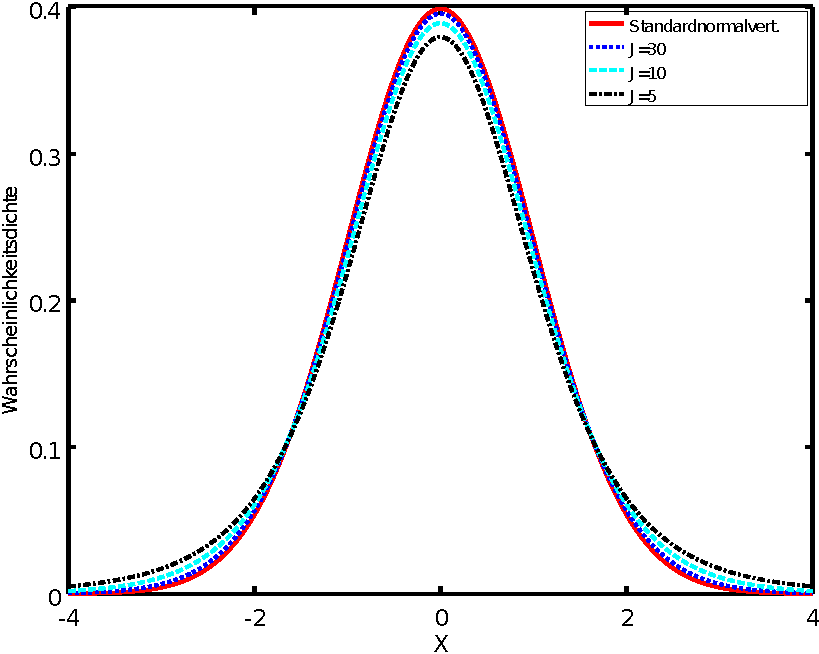
\includegraphics[width=100mm]{05_vorlesung/media/learn_Student_tpdf.pdf}
\caption{\label{studentt} Student-t Verteilungen für unterschiedliche Stichprobenumfänge.}
\end{center}
\end{figure}
Um zu verdeutlichen, wie sich die Gaußverteilung und die Student-t-Verteilung hinsichtlich
Breite und lange Ausläufer unterscheiden, haben wir hier dies im Vergleich berechnet.
Dabei haben wir bewusst ganz extrem wenig Freiheitsgrade gewählt, nämlich nur $5$.
Wir verwenden jetzt mal den empirischen Mittelwert und die empirische Standardabweichung,
die wir aus der Gesamtheit aller Stichproben gewonnen hatten, also $y = 41.57$
und $s = 4.88$. Daraus rechnen wir sowohl die Normalverteilung als auch die
Student-t-Verteilung für nur fünf Freiheitsgrade und erhalten eine größere Standardabweichung
und eine größere Kurtosis aus der Student-t-Verteilung:
\begin{center}
\begin{tabular}{l||c|c}
\hline
Verteilung & $\sigma$ & Kurt\\
\hline
Gauß &   4.88 &  2.99 \\
Student-t &  5.86 &  3.59 \\
\hline
\end{tabular}
\end{center}
Dementsprechend sind auch die Quantile größer.


Die Kurtosis
der Student-t Verteilungen nimmt Werte an, die um so größer werden, je flacher die Verteilungsdichte
ist, also je ausgeprägter die \textsl{Tails} sind, also je kleiner die Stichprobenumfänge bzw.\ die 
Anzahl der Freiheitsgrade sind.

%----

Das Vertrauensintervall zu einem Vertrauensniveau von $1 - \alpha$ für eine endlich große
Strichprobe mit Stichprobenumfang $J$ schätzen wir mit dem Quantil der Student-t-Verteilung ab.
Die Anzahl der Freiheitsgrade entspricht dem Stichprobenumfang abzüglich der Anzahl der zu
schätzenden Modellparameter, was in diesem Fall einer ist, also $\nu = J - 1$.



%---------------

Während für die Standardnormalverteilung das Quantil $z_{0.975} \; = \; 1.96$ beträgt, haben
wir aus der Student-t-Verteilung zu demselben Vertrauensniveau für $\nu = 50$ Freiheitsgrade
$t_{0.975, 50} \; = \; 2.01$ und für $\nu = 5$ Freiheitsgrade $t_{0.975, 5} \; = \; 2.57$.

\begin{figure}
\begin{center}
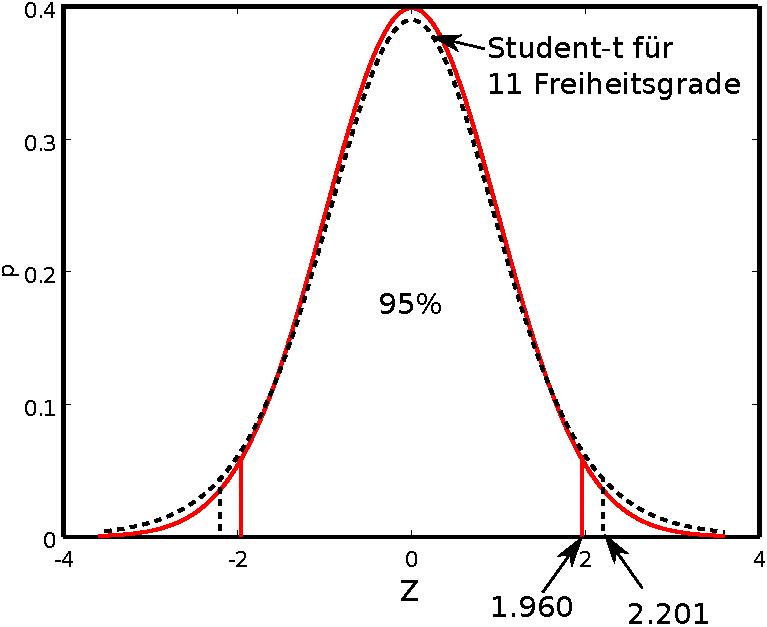
\includegraphics[width=100mm]{05_vorlesung/media/vertrauensintervall_nu_11.pdf}
\caption{\label{Vertrauensintervalle} Vertrauensintervalle in Vergleich für die 
Standardnormalverteilung (rote Kurve)
und die Student-t-Verteilung für $\nu = 11$ Freiheitsgrade (schwarze gestrichelte Kurve).}
\end{center}
\end{figure}
Für das zweiseitige, symmetrische Intervall verwenden wir das Quantil $t_{1-\alpha/2,\nu}$, so dass
wir folgendes Vertrauensintervall erhalten:
$$
[y - t_{1-\alpha/2,\nu} s, y + t_{1-\alpha/2,\nu} s]
$$
Die Breite wird durch die Anzahl der Freiheitgrade beeinflusst, je kleiner
die Anzahl der Freiheitsgrade ist, desto breiter wird das Intervall. Die beiden Abbn.~\ref{studentt}
und \ref{Vertrauensintervalle}
zeigen, dass die \textsl{Tails} einer Student-t-Verteilung für wenige Freiheitsgrade
deutlich breiter sind als bei der Standardnormalverteilung, folglich auch das
Vertrauensintervall breiter ist. In Abb.~\ref{Vertrauensintervalle} sind die Quantile für
ein Vertrauensniveau von $1 - \alpha = 0.95$ eingezeichnet.

Das \textsl{(vollständige) Messergebnis} geben wir an als
Schätzwert zur Größe $Y$ gemeinsam mit dem Vertrauensintervall.
Eine gebräuchliche Schreibweise ist
\begin{equation}
Y \; = \; y \, \pm \, t_{1-\alpha/2,\nu} s .
\label{vollstaendigesErgebKlassisch}
\end{equation}

Als nächstes befassen wir uns damit, das Vertrauensintervall des Mittelwertes abzuschätzen.
Dazu betrachten wir ein Beispiel, bei dem aus einer Grundgesamtheit mit den wahren
Werten $Y = 42$ und $\sigma = 7$ mehrere Stichproben genommen werden, beispielsweise $K = 15$,
wobei jede Stichprobe einen Umfang von $J = 25$ habe. Zu jeder der Stichproben $k = 1\dots K$
berechnen wir den Mittelwert $y_k$ und die empirische Standardabweichung $s_k$.

\begin{tabular}{c||c|c|c|c|c|c|c|c}
$k$   &  1     &    2   &    3   &   4    &    5   &   6    &   7    &   8   \\
\hline\hline
$y_k$ & 41.813 & 41.854 & 39.084 & 42.117 & 41.532 & 40.428 & 42.717 & 39.727\\
\hline
$s_k$ &  6.476 &  7.706 &  6.996 &  7.729 &  6.431 &  7.516 &  7.505 &  7.439\\
\end{tabular}

\vspace{3mm}

\begin{tabular}{c||c|c|c|c|c|c|c}
$k$   &  9     &    10  &   11   &   12   &   13   &   14   &   15  \\
\hline\hline
$y_k$ & 40.858 & 39.670 & 44.351 & 42.011 & 41.935 & 44.509 & 39.921\\
\hline
$s_k$ &  8.568 &  7.649 &  6.082 &  7.661 &  7.084 &  7.878 &  7.084\\
\end{tabular}

Der Mittelwert $\bar y$ der Mittelwerte liefert dann
$$
\bar y \; = \; \frac{1}{K} \sum\limits_{k=1}^K y_k \; = \; 41.502
$$
und die empirische Standardabweichung der Mittelwerte $y_k$ liefert
$$
\bar s \; = \; \sqrt{\frac{1}{K-1} \sum\limits_{k=1}^K (y_k \, - \, \bar y)^2 }
 \; = \; 1.606
$$
Das wiederholte Ziehen von Stichproben kann für so manche Anwendung kostspielig sein,
so dass es gilt die empirische Standardabweichung des Mittelwerts aus nur einer
Stichprobe abzuschätzen.
Dazu betrachten wir die Likelihood 
\begin{equation}
l(Y, \sigma | \{X_{1,1}, \dots, X_{1,J}\}) \; = \;
\prod\limits_{j=1}^J \frac{1}{\sqrt{2 \pi} \, \sigma}
 e^{- \frac{1}{2} \, \left( \frac{(X_{1,j} - Y)}{\sigma} \right)^2 } 
\label{LikelihoodY}
\end{equation}
und
setzten den Schätzer $y$ der Größe $Y$ als nahrhafte Null ein
\begin{equation}
l(Y, \sigma | \{X_{1,1}, \dots, X_{1,J}\}) \; = \;
\prod\limits_{j=1}^J \frac{1}{\sqrt{2 \pi} \, \sigma}
 e^{- \frac{1}{2} \, \left( \frac{(X_{1,j} - y) - (Y - y)}{\sigma} \right)^2 } 
\label{LikelihoodNahrhafteNull}
\end{equation}
d.h.
\begin{equation}
l(Y, \sigma | \{X_{1,1}, \dots, X_{1,J}\}) \; = \;
 \frac{1}{(\sqrt{2 \pi} \, \sigma)^J}
 e^{- \frac{1}{2} \, \sum\limits_{j=1}^J \left( \frac{(X_{1,j} - y) - (Y - y)}{\sigma} \right)^2 } .
\end{equation}
mit folgender Nebenrechnung für die Summe im Exponenten
$$
\arraycolsep=2.4pt\def\arraystretch{2}
\begin{array}{ll}
\sum\limits_{j=1}^J \left( (X_{1,j} - y) - (Y - y) \right)^2  & =
\sum\limits_{j=1}^J \left( (X_{1,j} - y)^2 + (Y - y)^2 - 2 (X_{1,j} - y) (Y - y) \right) \\
 & = \left( \sum\limits_{j=1}^J  (Y - y)^2\right) + 
 \left( \sum\limits_{j=1}^J  (X_{1,j} - y)^2\right) - 2 \sum\limits_{j=1}^J (X_{1,j} - y) (Y - y)\\
 & = J (Y - y)^2 + 
 \left( \sum\limits_{j=1}^J  (X_{1,j} - y)^2\right)
\end{array}
$$
und $\sum\limits_{j=1}^J (X_{1,j} - y) (Y - y) = 0$ wegen $J y = \sum\limits_{j=1}^J X_{1,j}$
gilt für die Likelihood folgende Proportionalität
\begin{equation}
l(Y, \sigma | \{X_{1,1}, \dots, X_{1,J}\}) \; \propto \;
 e^{- \frac{1}{2} \, J \, \left( \frac{(Y - y)}{\sigma} \right)^2 }
\label{LikelihoodmitJ}
\end{equation}
und wir definieren folgende Größe
\begin{equation}
\bar \sigma^2 \; := \; \frac{\sigma^2}{J}
\label{VarianzMittelwert}
\end{equation}
als \textsl{Varianz des Mittelwertes}.

Damit lässt sich Gl.~(\ref{LikelihoodmitJ}) umschreiben in
\begin{equation}
l(Y, \sigma | \{X_{1,1}, \dots, X_{1,J}\}) \; \propto \;
 e^{- \frac{1}{2} \, \left( \frac{(Y - y)}{\bar \sigma} \right)^2 } .
\end{equation}
Nun setzen wir in die Definitionsgleichung
der Varianz des Mittelwertes Gl.~(\ref{VarianzMittelwert}) bzw.\
die Wurzel daraus die empirisch ermittelten Werte unseres Beispiels ein:
\begin{equation}
\bar s \; = \; \frac{s}{\sqrt{J}}
\label{empirischeVarianzMittelwert}
\end{equation}

\begin{tabular}{c||c|c|c|c|c|c|c|c}
$k$   &  1     &    2   &    3   &   4    &    5   &   6    &   7    &   8   \\
\hline\hline
$\bar s_k$ &  1.295 &  1.541 &  1.399 &  1.546 &  1.286 &  1.503 &  1.501 &  1.488\\
\end{tabular}

\vspace{3mm}

\begin{tabular}{c||c|c|c|c|c|c|c}
$k$   &  9     &    10  &   11   &   12   &   13   &   14   &   15  \\
\hline\hline
$\bar s_k$ &  1.714 &  1.530 &  1.216 &  1.532 &  1.417 &  1.576 &  1.417\\
\end{tabular}

Jede einzelne Stichprobe liefert eine etwas unterschiedliche Abschätzung für die
Standardabweichung des Mittelwertes. Die Werte für $\bar s$ liegen mit $1.3$ bis $1.5$
knapp unter $1.6$. Es wird die Standardabweichung des Mittelwertes leicht unterschätzt, weil
der einzelne Stichprobenumfang mit $J = 25$ größer ist als die Anzahl der Stichproben mit
$K = 15$.

Das \textsl{Vertrauensintervall für die Schätzung des Mittelwertes} im Gegensatz zur
Schätzung des Einzelwertes ist damit
$$
[y - t_{1-\alpha/2,\nu} \bar s, y + t_{1-\alpha/2,\nu} \bar s]
$$
und in der Schreibweise als \textsl{vollständiges Messergebnis}
\begin{equation}
Y \; = \; y \, \pm \, t_{1-\alpha/2,\nu} \bar s .
\label{vollstaendigesErgebMittelwert}
\end{equation}


%===============


\section{t-Test - Mittelwerttest}


Nicht nur um die Qualität von schwarzem Bier (Stout) zu überprüfen, sondern ganz
allgemein, wird der t-Test eingesetzt, um zu testen, ob 
\begin{enumerate}
\item eine Stichprobe zu einer Grundgesamtheit gehört,
 deren Erwartungswert bekannt ist;
\item zwei Stichproben zur gleichen Grundgesamtheit gehören,
 deren Erwartungswert nicht bekannt ist, sondern deren jeweilige
 Mittelwerte miteinander verglichen werden.
\end{enumerate}

Sei $\mu_1$ der Erwartungswert der Grundgesamtheit zu Stichprobe 1 mit
Beobachtungen $(X_{1,1},\dots,$ $X_{1,J_1})$ und sei $\mu_2$ der Erwartungswert der 
zu Stichprobe 2 mit Beobachtungen $(X_{2,1}, \dots, X_{2,J_2})$.
Die Nullhypothese $H_0$ lautet, dass beide zu derselben Grundgesamtheit gehören,
was soviel bedeutet wie $\mu_1 = \mu_2$. Die Alternativhypothese $H_\mathrm{a}$
lautet, dass sie zu unterschiedlichen Grundgesamtheiten gehören,
was soviel bedeutet wie $\mu_1 \neq \mu_2$.

\begin{center}
\begin{tabular}{c|cl}
$H_0$ & $\mu_1 = \mu_2$ & beide Stichproben gehören derselben Grundgesamtheit an\\
\hline
$H_\mathrm{a}$ & $\mu_1 \neq \mu_2$ & beide Stichproben gehören unterschiedlichen Grundgesamtheiten an
\end{tabular}
\end{center}

Die Prüfgröße ist die Differenz der empirisch berechneten Mittelwerte normiert auf die
Standardabweichungen der Mittelwerte. Mit Gl.~(\ref{empirischeStd}) wird die
empirische Standardabweichung einer Stichprobe berechnet. Das in Tabelle 1 aufgeführte
Beispiel zeigt, dass die Mittelwerte deutlich weniger streuen, als die Werte innerhalb
einer einzelnen Stichprobe. Die Varianz des Mittelwertes einer Stichprobe wird gemäß
Gl.~(\ref{empirischeVarianzMittelwert}) darüber abgeschätzt, dass sie durch den Stichprobenumfang geteilt wird:
\begin{equation}
\bar s_i^2 \; = \; \frac{1}{J_i (J_i - 1)} \sum_{j=1}^{J_i} \, (X_{i,j} - y_i)^2
\end{equation}
Die Prüfgröße des t-Tests für den Vergleich der beiden Stichproben $i = 1,2$ ist wie folgt definiert
\begin{equation}
T \; = \; \frac{y_1 \, - \, y_2}{\sqrt{\bar s_1^2 + \bar s_2^2}}
\label{tTest}
\end{equation}
mit
\begin{equation}
y_i \; = \; \frac{1}{J_i}\sum_{j=1}^{J_i} \, X_{i,j} \qquad \mathrm{mit} \qquad
i = 1, 2
\end{equation}
Die Nullhypothese wird mit einem Signifikanzniveau von $\alpha = 0.05$ abgelehnt, wenn
der Betrag der Prüfgröße größer als das entsprechende Quantil der t-Verteilung ist
\begin{equation}
|T| \; > \; t_{1-\frac{1}{2} \alpha, \, \nu} \qquad \Rightarrow \qquad H_0 \; \; \mathrm{ablehnen}
\end{equation}


Für den $t$-Test mit zwei Stichproben wird unterschieden nach \textsl{gepoolten} und nicht \textsl{gepoolten}
Stichproben. Unter \textsl{gepoolten} Stichproben (\textsl{Samples}) versteht man diejenigen, deren Varianzen
im wesentlichen als gleich zu betrachten sind.
Die gemeinsame Anzahl der Freiheitsgrade für \textsl{gepoolte} Samples, die für die Wahl des $t$-Quantils gebraucht wird, ist
\begin{equation}
\nu \; = \; J_1 + J_2 - 2
\label{dofpooled}
\end{equation}
und für NICHT \textsl{gepoolte}
\begin{equation}
\nu \; = \;
 \frac{ \left(\frac{s_1^2}{J_1} +\frac{s_2^2}{J_2}\right)^2}{ 
  \frac{\left(\frac{s_1^2}{J_1}\right)^2}{J_1 - 1} + \frac{\left(\frac{s_2^2}{J_2}\right)^2}{J_2 - 1} } .
\label{dofnonpooled}
\end{equation}
Die Herleitung zur Berechnung der Anzahl der Freiheitsgrade für nicht gepoolte Stichproben
wird in Kapitel \ref{unsicherheitsfortpfLin} dran kommen. Gl.~(\ref{dofnonpooled}) wird auch
Satterthwaite'sche Gleichung genannt.

Bei $\nu = J_1 + J_2 - 2$ Freiheitsgraden, bei dem hier betrachteten Beispiel ist dies
$\nu = 98$ ist $t_{1-\frac{1}{2} \alpha, \, \nu} = t_{0.975, 98} = 1.985$.
Der Vergleich der ersten mit der zweiten Stichprobe aus Tabelle 1 liefert
$$
|T| \; = \; \frac{|40.79 \; - \; 43.08|}{\sqrt{\frac{1}{50} (4.83)^2 \; + \; \frac{1}{50} (5.52)^2}}
\; = \; 2.21  \; > \; 1.99
$$
dass die Mittelwerte der beiden Stichproben signifikant, auf einem Signifikanzniveau von
$\alpha = 0.05$, von einander abweichen und die Nullhypothese verworfen wird.

Betrachtet man jedoch einen größeren Vertrauensbereich, also anstelle von $95 \%$ einen
Bereich von $98 \%$, nimmt man also mehr aus dem Bereich der \textsl{Tails} hinzu, so
wird die Nullhypothese nicht verworfen. Auf einem Signifikanzniveau von nur
$\alpha = 0.02$ hat das Vertrauensintervall die Grenzen
$-t_{1-\frac{1}{2} \alpha, \, \nu} = -t_{0.99, 98} = -2.365$ und
$t_{1-\frac{1}{2} \alpha, \, \nu} = t_{0.99, 98} = 2.365$. Die
Nullhypothese wird für diese Wahl des Signifikanzniveaus nicht verworfen,
weil die Prüfgröße innerhalb des breiteren Intervalls mit
$|T| \; = \; 2.21 \; < \; 2.37$ liegt.

\begin{verbatim}
http://www.itl.nist.gov/div898/handbook/eda/section3/eda353.htm
\end{verbatim}

\section{Chi2-Verteilung und Varianztest}


Eine Verteilungsdichtefunktion, die die Verteilung der Quadrate einer
 normierten Zufallsgröße $Z$,
also die Verteilung der Varianzen einer Zufallsgröße $X$, beschreibt, ist die 
\textsl{Chi-Quadrat}-Verteilung.


Bisher haben wir uns damit befasst, wie eine Zufallsgröße $X$ streut.
Jetzt betrachten wir, wie die Streuung ihrerseits streut.
Wir betrachten eine Zufallsgröße, die zu einer normalverteilten Grundgesamtheit gehört.
\begin{quote}
$X$ sei eine eine normalverteilte Zufallsgröße mit Erwartungswert $\mu$ und Varianz $\sigma^2$
\end{quote}
d.h.
\begin{equation}
X \; \sim \; \mathcal{N}(\mu, \sigma).
\end{equation}
Werden einzelne kleinere Stichproben $X_i$ aus der Grundgesamtheit von $X$ entnommen, die
jeweils einen Stichprobenumfang $J_i$ haben und werden die jeweiligen Mittelwerte und
empirischen Varianzen berechnet
\begin{equation}
y_i \; = \; \frac{1}{J_i} \, \sum_{j=1}^{J_i} \, X_{i,j} \qquad
 s_i^2 \; = \; \frac{1}{J_i-1} \, \sum_{j=1}^{J_i} \, (X_{i,j} \, - \, y_i)^2
\end{equation}
so haben wir anhand der zuvor behandelten Beispiele festgestellt,
dass nicht nur die Mittelwerte $y_i$ sondern auch die Varianzen $s_i^2$ streuen.
Die Charakteristik der Verteilungsdichte der Varianzen hängt vom
Stichprobenumfang $J_i$ ab. Der Stichprobenumfang entspricht der Anzahl der Freiheitsgrade.

Gegeben sei eine Stichprobe $Z_1, \dots, Z_J$ unabhängiger Beobachtungen einer
standardnormalverteilten Zufallsgröße $Z$:
Dann ist die Summe der Quadrate der Beobachtungen $Q$ 
\begin{equation}
Q \; = \; \sum_{j=1}^J \, Z_j^2
\end{equation}
gemäß folgender Wahrscheinlichkeitsdichtefunktion verteilt
\begin{equation}
p(Q, J) \; = \; \frac{Q^{\frac{J}{2} - 1} \,
 e^{-\frac{Q}{2}}}{2^{\frac{J}{2}} \, \Gamma(\frac{J}{2})} \qquad Q > 0
\label{Chi2pdf}
\end{equation}
mit der Gammafunktion für natürliche Zahlen $\nu = J$, deren Definition im Abschnitt zuvor
als Gl.~(\ref{GammaHalfInt}) angegeben wurde.

Eine Schreibweise für die Aussage
\begin{quote}
$Q$ ist Chi2-verteilt
\end{quote}
ist
\begin{equation}
Q \; \sim \; \chi^2 .
\label{Chi2verteilt}
\end{equation}
Die Definition der $\chi^2$-Verteilungsdichtefunktion braucht nicht auswendig gelernt zu 
werden. Der Umgang mit den Quantiltabellen ist aber zu üben.
Wichtig zu wissen ist, dass die $\chi^2$-Verteilungs\-dichte\-funktion für
einen positiven Wertebereich gilt, sie ihr Maximum in der Nähe von $Q = J$ hat, sie um so
schiefer und breiter ist, je kleiner $J$ ist und die Verteilungsdichte der Varianzen
\begin{equation}
s_{\mu,i}^2 \; = \; \frac{1}{J_i} \, \sum_{j=1}^{J_i} \, (X_{i,j} \, - \, \mu)^2
\end{equation}
\begin{equation}
s_{\mu}^2 \; = \; \frac{1}{J} Q \, \sigma^2  \qquad \Leftrightarrow \qquad 
Q \; = \; J \, \left( \frac{s_{\mu}}{\sigma} \right)^2
\label{s2Q}
\end{equation}
liefert. Was in der Praxis hinsichtlich des Statistiktests, dem Chi2-Test, gebraucht wird,
ist das Verständnis wie die Tabellen verwendet werden
und für Methoden der Bayesischen Statistik erforderlichenfalls auch wie die
Funktionen der jeweils eingesetzten Numerik-/Statistik\-biblio\-theken zu benutzen sind. 

\begin{figure}
\begin{center}
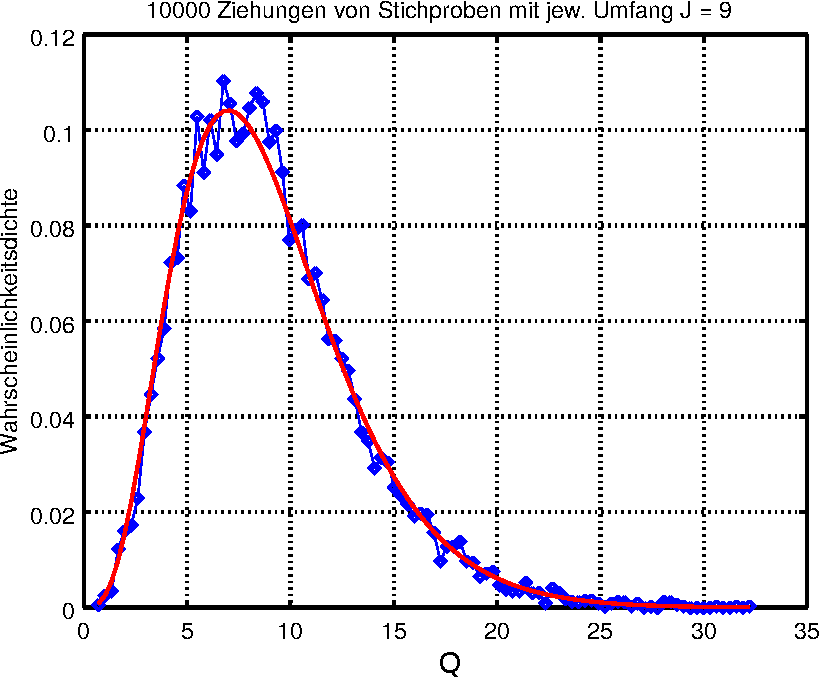
\includegraphics[width=75mm]{05_vorlesung/media/understandchi2_df9_final.pdf} \hspace{5mm}
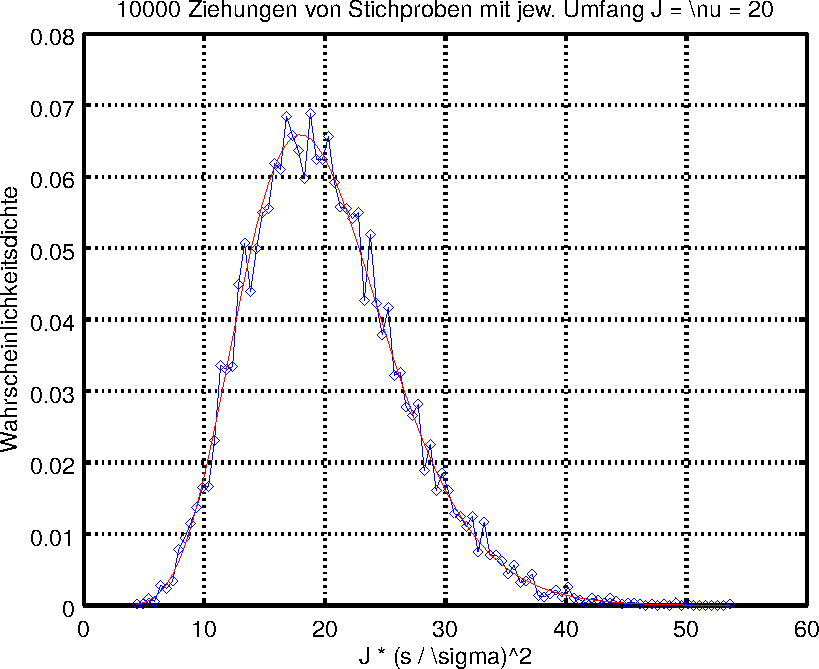
\includegraphics[width=75mm]{05_vorlesung/media/understandchi2_df20_final.pdf}
\caption{\label{ch2beispiele}$\chi^2$-Verteilung der normierten
Zufallsgröße $Q \; = \; J \, \left( \frac{s_{\mu}}{\sigma} \right)^2$ für
$s_{\mu}^2 \; = \; \frac{1}{J} \, \sum_{j=1}^{J} \, (X_{..,j} \, - \, \mu)^2$
für $J = 9$  (\textsl{links}) und $J = 20$ (\textsl{rechts}).}
\end{center}
\end{figure}

Abb.~\ref{ch2beispiele} zeigt zwei Beispiele für die Verteilungsdichte der Varianzen, zum einen
für $J = 9$ und zum anderen für $J = 20$. Mit
\begin{verbatim}
function understandchi2()
  Jz = 9;
  nbin = 100;
  n = 10000;
  d = zeros(n,1);
  for k=1:n
    x = randn(Jz,1);
    d(k) = sum(x.^2);
  end
  [haeuf, bin] = hist(d,nbin);
  Deltabin = bin(2)-bin(1);
  figure(1000);
  plot(bin,haeuf/(n*Deltabin),'bd-',bin,chi2pdf(bin,Jz),'r-');
  xlabel('J * (s / \sigma)^2', 'fontsize', 14);
  ylabel('Wahrscheinlichkeitsdichte', 'fontsize', 14);
  title([num2str(n) 'Stichprobenumfang J = \nu = ' num2str(Jz)], 'fontsize', 14);
  grid on;
  set(gca, 'fontsize', 14, 'linewidth', 2);
  print(1000,['understandchi2_df' num2str(Jz) '_solid.svg'],'-dsvg');
\end{verbatim}
wurden die Diagramme erzeugt. Die Verteilung der Grundgesamtheit ist die
Standardnormalverteilung mit $\mu = 0$ und $\sigma = 1$.
Eine Stichprobenentnahme wird mit \texttt{x = randn(Jz,1);} simuliert.

Wie bei der Quantildefinition für die Standardnormalverteilung und für die $t$-Verteilung
ist das Quantil der $\chi^2$-Verteilung die obere Integrationsgrenze
zur Gewinnung des Flächeninhalts der Verteilungsdichte. Dies quantifiziert die Wahrscheinlichkeit,
mit der für die Größe $Q$ Werte beobachtet werden, die kleiner sind als das Quantil.
Hier ist die untere Integrationsgrenze Null und nicht minus Unendlich, weil $Q$ per
Definitionem nur positive Werte haben kann, siehe Abb.~\ref{chi2quantil}.
\begin{figure}
\begin{center}
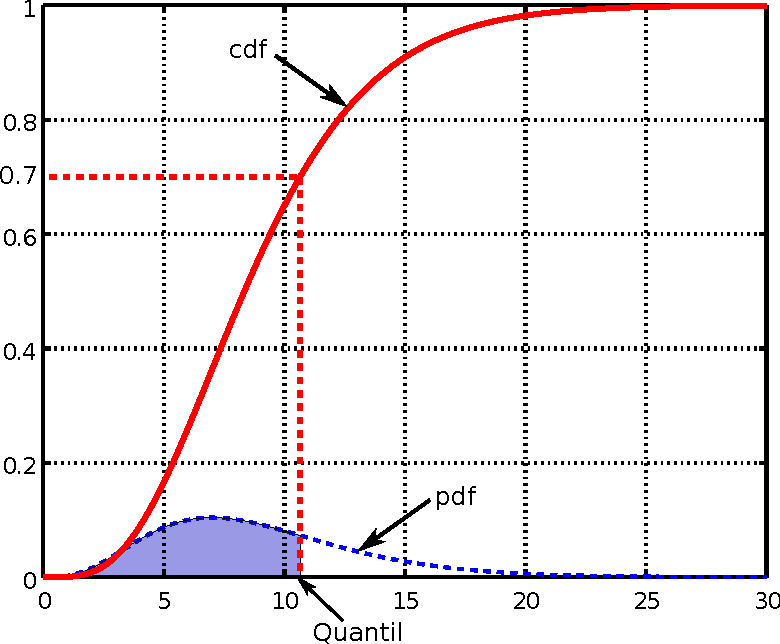
\includegraphics[width=100mm]{05_vorlesung/media/chiquadrat.pdf}
\caption{\label{chi2quantil}Wahrscheinlichkeitsverteilungsdichte (pdf) und
kumulierte Wahrscheinlichkeitsfunktion (cdf)
der normierten Varianzen, das Quantil wird $\chi^2$ genannt. Hier für 
$\nu = 9$ Freiheitgrade und $1 - \alpha = 0.7$, somit $\chi^2_{\nu, 1-\alpha} = 10.66$
dargestellt.}
\end{center}
\end{figure}
\begin{equation}
P(Q) \; = \; 
\int \limits_0^{\chi^2_{1-\alpha, \nu}}
p(Q^\prime, \nu) \; \operatorname{d} Q^\prime \; = \;
1 \, - \, \alpha
\label{chiQuadratQuantil}
\end{equation}
Für den $\chi^2$-Test wird, weil der Erwartungswert der Grundgesamtheit nicht bekannt ist,
die Varianz durch die empirische Varianz 
\begin{equation}
s_{\mu,i}^2 \; = \; \frac{1}{J_i} \, \sum_{j=1}^{J_i} \, (X_{i,j} \, - \, \mu)^2
\; \approx \; \frac{1}{J_i-1} \, \sum_{j=1}^{J_i} \, (X_{i,j} \, - \, y_i)^2
\; = \; s_i^2
\end{equation}
approximiert.
\begin{verbatim}
  for k=1:n
    x = randn(Jz,1);
    y = mean(x);
    d(k) = sum((x-y).^2);
  end
\end{verbatim}
Dann ist die Anzahl der Freiheitsgrade $\nu = J-1$ um einen vermindert,
weil der Mittelwert $y_i$ von den Werten $X_{i,j}$ abhängt. Die $\chi^2$-Verteilung
ist mit der Anzahl der Freiheitsgrade und nicht mit dem Stichprobenumfang zu verwenden
\begin{equation}
s^2 \; = \; \frac{1}{\nu} Q \, \sigma^2  \qquad \Leftrightarrow \qquad 
Q \; = \; \nu \, \left( \frac{s}{\sigma} \right)^2 ,
\label{s2Qempir}
\end{equation}
so dass die $\chi^2$-Verteilungsdichte, hier mit dem Funktionsaufruf
\texttt{chi2pdf} für $\nu = J-1$ zu verwenden ist:
\begin{verbatim}
  [haeuf, bin] = hist(d,nbin);
  Deltabin = bin(2)-bin(1);
  plot(bin,haeuf/(n*Deltabin),'bd-',bin,chi2pdf(bin,Jz-1),'r-');
  xlabel('(J-1) * (s / \sigma)^2', 'fontsize', 14);
\end{verbatim}

Für den Fall, den wir weiter oben betrachtet hatten, nämlich dass für den Erwartungswert
$\mu$ nicht sein Schätzer (der Mittelwert) verwendet wird, ist die Anzahl der
Freiheitsgrade gleich dem Stichprobenumfang.

Beim Chi-Quadrat-Test wird geprüft, ob die Varianz einer Stichprobe gleich einer
spezifizierten Varianz $\sigma_0^2$ ist. Wir formulieren die Hypothesen
\begin{center}
\begin{tabular}{c|cl}
$H_0$ & $\sigma^2 = \sigma_0^2$ & die Stichprobe gehört zu einer Grundgesamtheit mit der Varianz $\sigma_0^2$\\
\hline
$H_\mathrm{a}$ & $\sigma^2 \neq \sigma_0^2$ & die Stichprobe gehört nicht zu einer Grundgesamtheit mit der Varianz $\sigma_0^2$
\end{tabular}
\end{center}
Die Testgröße ist
\begin{equation}
T \; = \; \nu \, \left( \frac{s}{\sigma_0} \right)^2
\label{chi2testgroesse}
\end{equation}
Die Nullhypothese wird mit einem Signifikanzniveau von $\alpha$
verworfen, falls die Testgröße außerhalb des Intervalls liegt,
das durch die in Gl.~(\ref{chiQuadratQuantil}) definierten Quantile begrenzt wird, d.h.
\begin{equation}
T \; < \; \chi^2_{\alpha, \nu}  \qquad \mathrm{oder} \qquad
T \; > \; \chi^2_{1-\alpha, \nu} .
\end{equation}

\begin{verbatim}
http://www.itl.nist.gov/div898/handbook/eda/section3/eda358.htm
\end{verbatim} 

\section{Anwendung von Hypothesentests}

Anwendung finden die Hypothesentests im Bereich der Qualitätssicherung in der Produktion (siehe beispielsweise
zur Prüfung des Stout in der Guinessbrauerei schon vor 100 Jahren), oder im Bereich der Naturwissenschaften
(Biologie, Chemie, Pharmazie, Medizien) zum Nachweis von Substanzen. Es geht darum, dass zu bewerten ist,
mit welcher Wahrscheinlichkeit Beobachtungen zu welcher Verteilung gehören.
Einer Entscheidung liegen Regeln zugrunde. Mit dem t-Test haben wir die Regeln kennengelernt, über
die wir entscheiden, ob zwei Datensätze zu der gleichen gaußverteilten Grundgesamtheit - der gleichen
Normalverteilung mit demselben Erwartungswert gehören. 

Als nächstes wollen wir untersuchen, welche Fehler mit welcher Wahrscheinlichkeit dabei entstehen können.
Anschließend wollen wir uns ansehen, wie eine Stichprobe mit einer Toleranzvorgabe verglichen wird.
Die Toleranzvorgabe liefert ein Intervall, dessen Lage mit der Lage der Wahrscheinlichkeitsverteilung
der zu untersuchenden Stichprobe verglichen wird.

\subsection{Entscheidung bei Vergleich zweier Stichproben}
\begin{figure}
\begin{center}
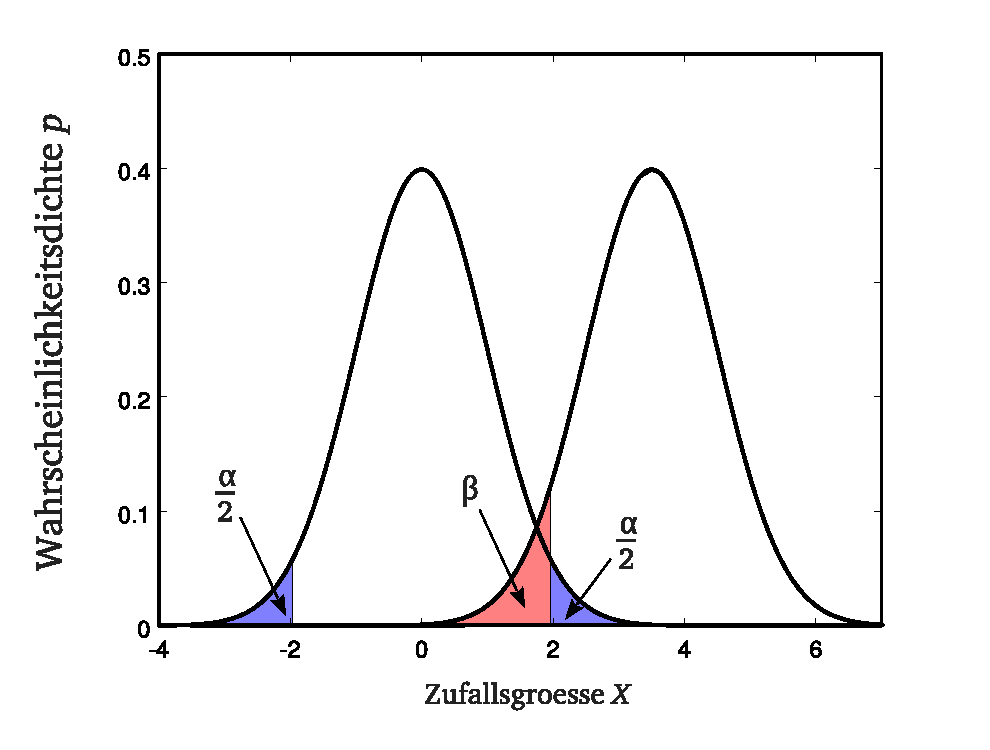
\includegraphics[width=100mm]{05_vorlesung/media/entscheidungsfehlertypen.pdf}
\caption{\label{entscheidungsfehler} Die Ereignisse (beobachtete Werte) aus der linken Wahrscheinlichkeitsdichteverteilung,
 die in deren \textsl{Tails} liegen, werden mit einem Signifikanzniveau von $\alpha$ verworfen.
 Die Ereignisse (beobachtete Werte) aus der rechten Wahrscheinlichkeitsdichteverteilung, die in dessen linkem
 \textsl{Tail} liegen, werden mit Wahrscheinlichkeit $\beta$ als der linken Wahrscheinlichkeit zugehörig
 erachtet.}
\end{center}
\end{figure}
Den Hypothesentests, die wir uns angesehen haben, ist gemeinsam, dass
\begin{enumerate}
\item eine Nullhypothese $H_0$ (evtl.\ auch eine Alternativhypothese $H_\mathrm{a}$)
aufgestellt wurde,
\item ein Signifikanzniveau $\alpha$ spezifiziert wurde,
\item eine Stichprobe mit einer Anzahl Freiheitsgrade $\nu$
genommen wurde und
\item anhand der vorher aufgestellten Entscheidungsregeln (Vergleich einer
Prüfgröße mit dem Quantil einer Wahrscheinlichkeitsdichteverteilung)
die Hypothese verworfen oder angenommen wurde.
\end{enumerate}
In der Entscheidungsregel werden durch Vorgabe eines Signifikanzniveaus Verwerfungsbereich
und Annahmebereich festgelegt. Das Signifikanzniveau ist dabei Komplementärwahrscheinlichkeit
(Gegenwahrscheinlichkeit) zum Vertrauensniveau, das ist die Wahrscheinlichkeit dafür
wie sicher die Hypothese ist.

Die Wahrscheinlichkeit, mit einem Hypothesentest eine falsche
Entscheidung zu treffen wird in zwei Klassen von Fehlern aufgeteilt, den
$\alpha$-Fehler oder den $\beta$-Fehler

\begin{center}
\begin{tabular}{M{3cm}|M{5.5cm}|M{5.5cm} N}
                 &     $H_0$ annehmen    &     $H_0$ ablehnen   \\[3pt]
\hline
$H_0$ ist wahr   & richtige Entscheidung, Wahrscheinlichkeit: $1-\alpha$ & Fehler 1.\ Art, Wahrscheinlichkeit $\alpha$ \\[3pt]
\hline
$H_0$ ist falsch & Fehler 2.\ Art, Wahrscheinlichkeit: $\beta$  & richtige Entscheidung, Wahrscheinlichkeit: $1-\beta$
\end{tabular}
\end{center}

Abb.~\ref{entscheidungsfehler} soll illustrieren, dass Beobachtungswerte, die zu einer
Grundgesamtheit mit einer Wahrscheinlichkeitsdichteverteilung mit Erwartungswert
$\mu_\mathrm{a} = 3.5$ gehören, per Hypothesentest einer Grundgesamtheit mit $\mu_0 = 0$
zugeordnet werden. Die Wahrscheinlichkeit für das Auftreten solcher Beobachtungen ist
dann $\beta$. Das Diagramm wurde mit folgendem Octaveskript erzeugt

\begin{verbatim}
function plot_entscheidungsfehler()
  dz = 0.02;
  lim = 7;
  z = [-lim:dz:lim];
  p1 = normpdf(z,0,1);
  t = 1.96;
  zleft = [-lim:dz:-t];
  pleft = normpdf(zleft,0,1);
  zright = [t:dz:lim];
  pright = normpdf(zright,0,1);
  mu2 = 3.5;
  p2 = normpdf(z+mu2,mu2,1);
  zbeta = [mu2-lim:dz:t];
  pbeta = normpdf(zbeta,mu2,1);
  figure(200); hold on;
  area( zleft, pleft, 'Facecolor', [0.5 0.5 1]);
  area( zright, pright, 'Facecolor', [0.5 0.5 1]);
  area( zbeta, pbeta, 'Facecolor', [1 0.5 0.5]);
  plot( z, p1, 'k-', 'linewidth', 2);
  plot( z+mu2, p2, 'k--', 'linewidth', 2);
  xlabel('X', 'fontsize', 14);
  ylabel('p', 'fontsize', 14);
  axis([-4 7 0 0.5]);
  set(gca, 'fontsize', 14);
  hold off;
  print(200, 'entscheidungsfehler.svg', '-dsvg');
end
\end{verbatim}

\subsection{Konformitätswahrscheinlichkeiten}
Nachdem wir gesehen haben wie wir zwei Hypothesen über die Lage zweier Wahrscheinlichkeitsdichteverteilungen
verglichen haben, befassen wir uns jetzt mit dem Vergleich eines Intervalls, einem Toleranzintervall, mit einer
Wahrscheinlichkeitsdichteverteilung. Für die Fertigung werden in den Konstruktionszeichnungen zu den Merkmalen
von Bauteilen die Toleranzen eingetragen, innerhalb derer die Merkmale des Werkstücks liegen müssen. Wie nun
bewertet man nach Fertigstellung des Werkstücks, ob ein Merkmal innerhalb einer Toleranzvorgabe liegt? Ein Merkmal
wird durch einen Messvorgang geprüft. Der Messvorgang liefert ein Ergebnis: Einen Zahlenwert für das Merkmal und
ein Überdeckungsintervall zusammen mit einem Vertrauensniveau. Anstelle von Überdeckungsintervall und Vertrauensniveau
kann auch direkt eine Wahrscheinlichkeitsdichteverteilung angegeben werden, ist aber sehr unüblich in der industriellen
Praxis. Für die Bewertung, ob das gefertigte Werkstück mit der Vorgabe der Konstruktion übereinstimmt, konform ist,
werden Messergebnis und Toleranzvorgabe verglichen.

Als Ergänzung zum \glqq Guide of Uncertainty\grqq gibt es das Dokument
\textsl{Evaluation of measurement data - The role of measurement uncertainty in conformity assessment},
das darlegt, wie Konformitätsbewertungen vorzunehem sind.
\begin{verbatim}
https://www.bipm.org/utils/common/documents/jcgm/JCGM_106_2012_E.pdf
\end{verbatim}
Dort heißt es in Paragraph 7.1.1
\begin{quote}
An item conforms to a specified requirement if the true value of its associated property $Y$ lies in the tolerance
interval. Knowledge of $Y$ is conveyed by a probability density function $p(y|{X_1,\dots,X_J})$
so that a statement of conformity is always an inference,
with some probability of being true. Denoting the set of permissible (conforming) values
$Y$ by $C$, the conformance probability, denoted by $p_\mathrm{c}$, is given by
\begin{equation}
	p_\mathrm{c} = P(Y \in C | {X_1,\dots,X_J}) = \int\limits_C p(y|{X_1,\dots,X_J}) \mathrm{d}y.
\end{equation}
\end{quote}
Im Originaldokument werden Sie eine etwas andere Schreibweise für die Bezeichner in der Formel vorfinden.
Hier ist es so aufgeschrieben, wie es zu der Notation innerhalb dieses Vorlesungsskriptes, insbesondere
zu Kapitel \ref{KonzepteinverseProbleme}, passt.
Für die Toleranz wird in der Richtlinie zur Konformitätsbewertung zur Wahrung der Allgemeingültigkeit
eine Menge $C$ angegeben. Falls die Größe $Y$ eine skalarwertige Größe wie bei dem Beispiel, anhand dessen
wir in Kapitel \ref{KonzepteinverseProbleme} das Prinzip der bayesischen Statistik illustriert haben,
so steht $C$ für ein Intervall $C = [y_\mathrm{L}, y_\mathrm{U}]$. Dabei sollen der Index L für \glqq lower
limit\grqq ~und der Index U für \glqq upper limit\grqq ~stehen.

Die Wahrscheinlichkeit $p_\mathrm{c}$, dass die Beobachtungen ${X_1,\dots,X_J}$ innerhalb des Toleranzintervalls
$C = [y_\mathrm{L}, y_\mathrm{U}]$ liegen, ist
\begin{equation}
	p_\mathrm{c} =  \int\limits_{y_\mathrm{L}}^{y_\mathrm{U}} p(y|{X_1,\dots,X_J}) \mathrm{d}y.
\end{equation}
Für den Fall, dass von einer normalverteilten Stichprobe ausgegangen werden kann und dass eine Einzelgröße
vorliegt, wird auch der Stichprobe ${X_1,\dots,X_J}$ der Schätzer $\bar y$ aus einfacher Mittelwertbildung
gewonnen ($\bar y = \sum_{j=1}^J X_j$) und die Varianz als empirische Varianz $s$ aus
$s = \frac{1}{J-1}\sum (X_j - \bar y)^2$ und für die Wahrscheinlichkeitsdichte $p$ die Gaußverteilung:
\begin{equation}
	p_\mathrm{c} = \frac{1}{\sqrt{2 \pi} s} \int\limits_{y_\mathrm{L}}^{y_\mathrm{U}} 
	e^{-\frac{1}{2}\left(\frac{y - \bar y}{s}\right)^2} \mathrm{d}y
\end{equation}
Die Größe $\frac{y - \bar y}{s}$ ist eine normierte Zufallsgröße. Die Integrationsgrenzen können gleichfalls
normiert werden: $z = \frac{y - \bar y}{s}$, $z_\mathrm{L} = \frac{y_\mathrm{L} - \bar y}{s}$ und
$z_\mathrm{U} = \frac{y_\mathrm{U} - \bar y}{s}$, so dass die Tabellenwerke oder Bibliotheksfunktion
für die gauß'sche Fehlerfunktion (\textsl{error function}) wie folgt verwendet werden kann:
\begin{equation}
p_\mathrm{c} = \frac{1}{\sqrt{2 \pi}} \int\limits_{-\infty}^{z_\mathrm{U}} 
	e^{-\frac{1}{2} z^2} \mathrm{d}z - 
	\frac{1}{\sqrt{2 \pi}} \int\limits_{-\infty}^{z_\mathrm{L}} e^{-\frac{1}{2} z^2} \mathrm{d}z
\end{equation}
d.h.
\begin{equation}
	p_\mathrm{c} = \mathrm{erf}(z_\mathrm{U}) - \mathrm{erf}(z_\mathrm{L}).
\end{equation}


%\bibliography{$BIBLIO/math}
%\bibliographystyle{unsrt}


\section{Übungsaufgaben zum Selbststudium}
\label{AufgVorl5}

\textbf{Aufgabe 1}\\

Probieren Sie anhand von Beobachtungen, die Sie mit Hilfe eines Generators, der
normalverteilte Zufallszahlen liefert, den Kolmogorow-Smirnow-Test, kurz KS-Test, aus.

In Matlab/Gnu-Octave könnten Sie dies beispielsweise wie folgt realisieren:
\begin{verbatim}
  J1 = 2000; % Stichprobenumfang
  mu1 = 23; % Erwartungswert der Zufallsgroesse
  s1 = 3;   % Wurzel aus dem Erwartungswert fuer die Varianz
  Xarray = s1*randn(J1,1) + mu1;
\end{verbatim}
Das Sortieren mit Matlab/Gnu-Octave können Sie mit
\begin{verbatim}
  [xsort, isort] = sort(Xarray, 'ascend');
\end{verbatim}
und die Wahrscheinlichkeiten mit
\begin{verbatim}
  h = [1:J1]'/J1;
\end{verbatim}
berechnen.

\begin{enumerate}
\item Verwenden Sie nicht die {\`a} priori eingesetzten Erwartungswerte,
 sondern Mittelwert \texttt{y = mean(Xarray)} und empirische Standardabweichung
 \texttt{s = std(Xarray)}, um die Funktion $P(X)$ aus Gl.~(\ref{cdfKS})
 zu realisieren. Berechnen Sie die relativen Häufigkeiten $H$ gemäß
 Gl.~(\ref{cdfH}), sowie den in Gl.~(\ref{KSpruefgroesse}) definierten
 Schwellwert
  $$K_{\alpha, J}$$
 zu einem Signifikanzniveau von $\alpha = 0.05$,
 wobei $J$ der Stichprobenumfang ist.
 Führen Sie den Test mit den von Ihnen erzeugten Zufallswerten durch.
\item Erzeugen Sie einen zusätzlichen Satz von Zufallszahlen, beispielsweise mit den
 Werten \texttt{mu2 = 35} und \texttt{s2 = 5}. Wählen Sie für diese einen
 deutlich kleineren Stichprobenumfang. Führen Sie den KS-Test für die
 vereinigten Zufallszahlenarrays durch und tun Sie so, als ob Sie nicht
 wüssten, dass dies keine gemeinsame Grundgesamtheit ist.
\end{enumerate}



\textbf{Aufgabe 2}

Gegeben seien zwei Stichproben

Stichprobe 1:

\begin{tabular}{|c|c|c|c|c|}
\hline
21 & 33 & 19 & 39 & 7\\
\hline
\end{tabular}

Stichprobe 2:

\begin{tabular}{|c|c|c|c|c|c|c|c|c|}
\hline
53 & 69 & 63 & 47 & 49 & 44 & 47 & 44 & 38\\
\hline
\end{tabular}

\begin{enumerate}
\item[a)] Geben Sie zu jeder der beiden Stichproben die Mittelwerte und Standardabweichungen an.
\item[b)] Prüfen Sie auf einem Signifikanzniveau von $\alpha = 0.05$ die Hypothese $H_0$,
 ob beide Stichproben zu einer Grundgesamtheit
 mit demselben Erwartungswert $\mu$ gehören. Geben Sie dazu die Formel und den Wert
 der Testgröße an und vergleichen Sie diese mit dem entsprechenden Quantil der für diesen
 Test zu verwendenden Verteilung. Mit welcher Verteilung ist dieser Test durchzuführen?
\item[c)] Prüfen Sie auf einem Signifikanzniveau von $\alpha = 0.05$ die Hypothese $H_0$,
 ob die zweite Stichprobe zu einer Grundgesamtheit
 mit der Standardabweichung $\sigma_0 = 6$ gehört. Geben Sie dazu die Formel und den Wert
 der Testgröße an und vergleichen Sie diese mit dem entsprechenden Quantil der für diesen
 Test zu verwendenden Verteilung. Mit welcher Verteilung ist dieser Test durchzuführen?
 Führen Sie nur den einseitigen Test durch, das heißt prüfen Sie nur bezüglich
 des rechten \textsl{Tail} der Verteilungsdichte.
\item[d)] Führen Sie denselben Test wie in (c) durch, aber dieses Mal für $\sigma_0 = 9$.
\end{enumerate}

Verwenden Sie die auf den folgenden Seiten abgedruckten Quantiltabellen.

\pagebreak

\section{Quantiltabellen}

\subsection{Quantile der Student-t Verteilung}
\begin{tabular}{c||c|c|c|c|c|}
d.o.f & \multicolumn{5}{c|}{Wahrscheinlichkeit}\\
\hline
$\nu$ & 0.995 & 0.990 & 0.975 & 0.950 & 0.800 \\ 
\hline\hline
2 & 9.925 & 6.965 & 4.303 & 2.920 & 1.061 \\ 
\hline
3 & 5.841 & 4.541 & 3.182 & 2.353 & 0.978 \\ 
\hline
4 & 4.604 & 3.747 & 2.776 & 2.132 & 0.941 \\ 
\hline
5 & 4.032 & 3.365 & 2.571 & 2.015 & 0.920 \\ 
\hline
6 & 3.707 & 3.143 & 2.447 & 1.943 & 0.906 \\ 
\hline
7 & 3.499 & 2.998 & 2.365 & 1.895 & 0.896 \\ 
\hline
8 & 3.355 & 2.896 & 2.306 & 1.860 & 0.889 \\ 
\hline
9 & 3.250 & 2.821 & 2.262 & 1.833 & 0.883 \\ 
\hline
10 & 3.169 & 2.764 & 2.228 & 1.812 & 0.879 \\ 
\hline
11 & 3.106 & 2.718 & 2.201 & 1.796 & 0.876 \\ 
\hline
12 & 3.055 & 2.681 & 2.179 & 1.782 & 0.873 \\ 
\hline
13 & 3.012 & 2.650 & 2.160 & 1.771 & 0.870 \\ 
\hline
14 & 2.977 & 2.624 & 2.145 & 1.761 & 0.868 \\ 
\hline
15 & 2.947 & 2.602 & 2.131 & 1.753 & 0.866 \\ 
\hline
16 & 2.921 & 2.583 & 2.120 & 1.746 & 0.865 \\ 
\hline
17 & 2.898 & 2.567 & 2.110 & 1.740 & 0.863 \\ 
\hline
18 & 2.878 & 2.552 & 2.101 & 1.734 & 0.862 \\ 
\hline
19 & 2.861 & 2.539 & 2.093 & 1.729 & 0.861 \\ 
\hline
20 & 2.845 & 2.528 & 2.086 & 1.725 & 0.860 \\ 
\hline
21 & 2.831 & 2.518 & 2.080 & 1.721 & 0.859 \\ 
\hline
22 & 2.819 & 2.508 & 2.074 & 1.717 & 0.858 \\ 
\hline
23 & 2.807 & 2.500 & 2.069 & 1.714 & 0.858 \\ 
\hline
24 & 2.797 & 2.492 & 2.064 & 1.711 & 0.857 \\ 
\hline
25 & 2.787 & 2.485 & 2.060 & 1.708 & 0.856 \\ 
\hline
\end{tabular}
\hspace{7mm}
\begin{tabular}{c||c|c|c|c|c|}
d.o.f & \multicolumn{5}{c|}{Wahrscheinlichkeit}\\
\hline
$\nu$ & 0.995 & 0.990 & 0.975 & 0.950 & 0.800 \\ 
\hline\hline
26 & 2.779 & 2.479 & 2.056 & 1.706 & 0.856 \\ 
\hline
27 & 2.771 & 2.473 & 2.052 & 1.703 & 0.855 \\ 
\hline
28 & 2.763 & 2.467 & 2.048 & 1.701 & 0.855 \\ 
\hline
29 & 2.756 & 2.462 & 2.045 & 1.699 & 0.854 \\ 
\hline
30 & 2.750 & 2.457 & 2.042 & 1.697 & 0.854 \\ 
\hline
31 & 2.744 & 2.453 & 2.040 & 1.696 & 0.853 \\ 
\hline
32 & 2.738 & 2.449 & 2.037 & 1.694 & 0.853 \\ 
\hline
33 & 2.733 & 2.445 & 2.035 & 1.692 & 0.853 \\ 
\hline
34 & 2.728 & 2.441 & 2.032 & 1.691 & 0.852 \\ 
\hline
35 & 2.724 & 2.438 & 2.030 & 1.690 & 0.852 \\ 
\hline
36 & 2.719 & 2.434 & 2.028 & 1.688 & 0.852 \\ 
\hline
37 & 2.715 & 2.431 & 2.026 & 1.687 & 0.851 \\ 
\hline
38 & 2.712 & 2.429 & 2.024 & 1.686 & 0.851 \\ 
\hline
39 & 2.708 & 2.426 & 2.023 & 1.685 & 0.851 \\ 
\hline
40 & 2.704 & 2.423 & 2.021 & 1.684 & 0.851 \\ 
\hline
41 & 2.701 & 2.421 & 2.020 & 1.683 & 0.850 \\ 
\hline
42 & 2.698 & 2.418 & 2.018 & 1.682 & 0.850 \\ 
\hline
43 & 2.695 & 2.416 & 2.017 & 1.681 & 0.850 \\ 
\hline
44 & 2.692 & 2.414 & 2.015 & 1.680 & 0.850 \\ 
\hline
45 & 2.690 & 2.412 & 2.014 & 1.679 & 0.850 \\ 
\hline
46 & 2.687 & 2.410 & 2.013 & 1.679 & 0.850 \\ 
\hline
47 & 2.685 & 2.408 & 2.012 & 1.678 & 0.849 \\ 
\hline
48 & 2.682 & 2.407 & 2.011 & 1.677 & 0.849 \\ 
\hline
49 & 2.680 & 2.405 & 2.010 & 1.677 & 0.849 \\ 
\hline
50 & 2.678 & 2.403 & 2.009 & 1.676 & 0.849 \\ 
\hline
\end{tabular}


\subsection{Quantile der $\chi^2$-Verteilung}

\begin{small}
\begin{tabular}{c||c|c|c|c|c|}
 & \multicolumn{5}{c|}{Wahrscheinlichkeit}\\
\hline
$\nu$ & 0.995 & 0.990 & 0.975 & 0.950 & 0.800 \\ 
\hline\hline
2 & 10.597 & 9.210 & 7.378 & 5.991 & 3.219 \\ 
\hline
3 & 12.838 & 11.345 & 9.348 & 7.815 & 4.642 \\ 
\hline
4 & 14.860 & 13.277 & 11.143 & 9.488 & 5.989 \\ 
\hline
5 & 16.750 & 15.086 & 12.833 & 11.070 & 7.289 \\ 
\hline
6 & 18.548 & 16.812 & 14.449 & 12.592 & 8.558 \\ 
\hline
7 & 20.278 & 18.475 & 16.013 & 14.067 & 9.803 \\ 
\hline
8 & 21.955 & 20.090 & 17.535 & 15.507 & 11.030 \\ 
\hline
9 & 23.589 & 21.666 & 19.023 & 16.919 & 12.242 \\ 
\hline
10 & 25.188 & 23.209 & 20.483 & 18.307 & 13.442 \\ 
\hline
11 & 26.757 & 24.725 & 21.920 & 19.675 & 14.631 \\ 
\hline
12 & 28.300 & 26.217 & 23.337 & 21.026 & 15.812 \\ 
\hline
13 & 29.819 & 27.688 & 24.736 & 22.362 & 16.985 \\ 
\hline
14 & 31.319 & 29.141 & 26.119 & 23.685 & 18.151 \\ 
\hline
15 & 32.801 & 30.578 & 27.488 & 24.996 & 19.311 \\ 
\hline
16 & 34.267 & 32.000 & 28.845 & 26.296 & 20.465 \\ 
\hline
17 & 35.718 & 33.409 & 30.191 & 27.587 & 21.615 \\ 
\hline
18 & 37.156 & 34.805 & 31.526 & 28.869 & 22.760 \\ 
\hline
19 & 38.582 & 36.191 & 32.852 & 30.144 & 23.900 \\ 
\hline
20 & 39.997 & 37.566 & 34.170 & 31.410 & 25.038 \\ 
\hline
21 & 41.401 & 38.932 & 35.479 & 32.671 & 26.171 \\ 
\hline
22 & 42.796 & 40.289 & 36.781 & 33.924 & 27.301 \\ 
\hline
23 & 44.181 & 41.638 & 38.076 & 35.172 & 28.429 \\ 
\hline
24 & 45.559 & 42.980 & 39.364 & 36.415 & 29.553 \\ 
\hline
25 & 46.928 & 44.314 & 40.646 & 37.652 & 30.675 \\ 
\hline
\end{tabular}
\hspace{2mm}
\begin{tabular}{c||c|c|c|c|c|}
 & \multicolumn{5}{c|}{Wahrscheinlichkeit}\\
\hline
$\nu$ & 0.995 & 0.990 & 0.975 & 0.950 & 0.800 \\ 
\hline\hline
26 & 48.290 & 45.642 & 41.923 & 38.885 & 31.795 \\ 
\hline
27 & 49.645 & 46.963 & 43.195 & 40.113 & 32.912 \\ 
\hline
28 & 50.993 & 48.278 & 44.461 & 41.337 & 34.027 \\ 
\hline
29 & 52.336 & 49.588 & 45.722 & 42.557 & 35.139 \\ 
\hline
30 & 53.672 & 50.892 & 46.979 & 43.773 & 36.250 \\ 
\hline
31 & 55.003 & 52.191 & 48.232 & 44.985 & 37.359 \\ 
\hline
32 & 56.328 & 53.486 & 49.480 & 46.194 & 38.466 \\ 
\hline
33 & 57.648 & 54.776 & 50.725 & 47.400 & 39.572 \\ 
\hline
34 & 58.964 & 56.061 & 51.966 & 48.602 & 40.676 \\ 
\hline
35 & 60.275 & 57.342 & 53.203 & 49.802 & 41.778 \\ 
\hline
36 & 61.581 & 58.619 & 54.437 & 50.998 & 42.879 \\ 
\hline
37 & 62.883 & 59.893 & 55.668 & 52.192 & 43.978 \\ 
\hline
38 & 64.181 & 61.162 & 56.896 & 53.384 & 45.076 \\ 
\hline
39 & 65.476 & 62.428 & 58.120 & 54.572 & 46.173 \\ 
\hline
40 & 66.766 & 63.691 & 59.342 & 55.758 & 47.269 \\ 
\hline
41 & 68.053 & 64.950 & 60.561 & 56.942 & 48.363 \\ 
\hline
42 & 69.336 & 66.206 & 61.777 & 58.124 & 49.456 \\ 
\hline
43 & 70.616 & 67.459 & 62.990 & 59.304 & 50.548 \\ 
\hline
44 & 71.893 & 68.710 & 64.201 & 60.481 & 51.639 \\ 
\hline
45 & 73.166 & 69.957 & 65.410 & 61.656 & 52.729 \\ 
\hline
46 & 74.437 & 71.201 & 66.617 & 62.830 & 53.818 \\ 
\hline
47 & 75.704 & 72.443 & 67.821 & 64.001 & 54.906 \\ 
\hline
48 & 76.969 & 73.683 & 69.023 & 65.171 & 55.993 \\ 
\hline
49 & 78.231 & 74.919 & 70.222 & 66.339 & 57.079 \\ 
\hline
50 & 79.490 & 76.154 & 71.420 & 67.505 & 58.164 \\ 
\hline
\end{tabular}
\end{small}



